\chapter{Informative Seafloor Exploration}
\lhead{Informative Seafloor Exploration}
\label{InformativeSeafloorExploration}

	The Gaussian process based inference model for benthic habitat mapping devised in Chapter \ref{BenthicHabitatMapping} provides a Bayesian framework for habitat inference and prediction. With such an inference model, this chapter proceeds to develop an informative path planning policy for benthic habitat mapping.
	
	In order to devise an informative path planning policy, it is important to select an appropriate acquisition criterion which measures the desirability of traversing a particular candidate path. Section \ref{Background:RelatedWork} provided an outline of related investigations on various acquisition functions for informative path planning in the benthic habitat mapping context, which motivated the need for a measure of mutual information. Such a measure would allow inference based on the \textit{essential} information contained in any given sub-region of interest. The mutual information criterion can then be employed as the acquisition function for informative path planning, in order to evaluate and thus compare the desirability of visiting candidate regions and locations.
	
	Nevertheless, as Gaussian process classifiers lack analytical forms for the \textit{predictive} joint distribution of target labels, any mutual information measure derived from the predictive joint distribution must rely on numerical estimation techniques. As such, estimating joint prediction information entropy requires a Monte Carlo sampling based approach. Section \ref{InformativeSeafloorExploration:MCPIE} describes such a mutual information criterion, hereby named Monte Carlo Predictive Information Entropy (MCPIE).
	
	However, a Monte Carlo approach suffers several drawbacks, such as computational complexity and limited estimation accuracy. Instead, this thesis proposes a new and alternative mutual information measure, Linearised Model Differential Entropy (LMDE), that is more computationally tractable than MCPIE. Instead of focusing on the \textit{predictive} joint distribution, LMDE focuses on the \textit{model} joint distribution by utilising the \textit{latent} joint distribution, where inference remains analytically tractable. Section \ref{InformativeSeafloorExploration:LMDE} defines and derives LMDE as an appropriate form of mutual information. Specifically, it regularises between reducing mutual bias and mutual uncertainty through taking advantage of both the latent mean and covariance structure, as well as the non-Gaussian likelihood response. Tractability of the approach is further improved through a linearisation approximation on such an acquisition criterion.
	
	Section \ref{InformativeSeafloorExploration:ComparisonMutualEntropyMeasures} proceeds to demonstrate the two mutual entropy measures through example datasets. Interpretation of the experimental results provides an intuitive understanding of their differences in time complexity, accuracy, and most importantly, their properties.
	
	Section \ref{InformativeSeafloorExploration:RecedingHorizonFormulation} then formulates a receding horizon approach to informative path planning. This provides a simple yet effective framework for a large scale exploration task such as seafloor exploration for benthic habitat mapping. In particular, the receding horizon formulation strikes a balance between exploring in a non-myopic way and doing so with reasonable tractability constraints.
	
	Finally, Section \ref{InformativeSeafloorExploration:ScottReef} assesses the performance of various approaches to informative seafloor exploration for benthic habitat mapping. Multiple acquisition criteria are tested under both the receding horizon approach and a myopic greedy approach, which verifies the benefits of linearised model differential entropy under the receding horizon formulation. Under a mapping accuracy criterion, simulations over the Scott Reef dataset demonstrates that LMDE acquisition outperform other criterions, with MCPIE acquisition following closely in performance.
		
	\section{Monte Carlo Predictive Information Entropy}
	\label{InformativeSeafloorExploration:MCPIE}
	
		This section introduces the Monte Carlo predictive information entropy (MCPIE) of Gaussian process classifiers. Monte Carlo sampling methods provide a way to estimate the joint predictive entropy through considering the joint distributions of the latent function at the query points.
	
		Monte Carlo sampling, as its name suggests, involve using sampled draws from a particular distribution to estimate a certain quantity that can be characterised by the distribution. In the MCPIE case, the distribution to be sampled from is the latent GP process of the GP classifier, whose moments are analytically tractable, and the quantity to be estimated is the \textit{joint} predictive information entropy of the query points. A brief description of the method is provided for both binary and multiclass classification.
		
		\subsection{Binary Classification}
		\label{InformativeSeafloorExploration:MCPIE:Binary}
		
			Suppose a Gaussian process classifier has been trained under \textit{any} approximation technique with respect to a training set $\mathcal{D} = \{X, \bvec{y}\} = \{[ \bvec{x}_{1}, \bvec{x}_{2}, \dots, \bvec{x}_{n}]^{T}, [y_{1}, y_{2}, \dots, y_{n}]^{T}\}$ with $n$ training points. It is known that the latent function $f(\bvec{x})$ is distributed as a GP with a particular predictive mean $m(\bvec{x})$ and covariance $k(\bvec{x}, \bvec{x}')$ once conditioned on the training data \eqref{Equation:PredictiveLatentBinaryGP}. Note that this chapter will omit explicitly notating the training data and query data that was conditioned upon, as well as the learned hyperparameters $\vec{\uptheta}$, unless otherwise stated. \begin{equation}
				f(\bvec{x}) \sim \mathcal{GP}(m(\bvec{x}), k(\bvec{x}, \bvec{x}'))
			\label{Equation:PredictiveLatentBinaryGP}
			\end{equation}
			
			Let $X^{\star} = [ \bvec{x}^{\star}_{1}, \bvec{x}^{\star}_{2}, \dots, \bvec{x}^{\star}_{n^{\star}}]^{T}$ denote the collection of $n^{\star}$ query points for which inference is to be performed upon. Denote $\bvec{f}^{\star}$ the vector of latent function values $f^{\star}_{i} = f(\bvec{x}^{\star}_{i})$ at each query point. By definition of a GP, $\bvec{f}^{\star}$ is multivariate Gaussian distributed with corresponding means $\mu^{\star}_{i} = m(\bvec{x}^{\star}_{i})$ and covariances $\Sigma^{\star}_{ij} = k(\bvec{x}^{\star}_{i}, \bvec{x}^{\star}_{j})$ \eqref{Equation:BinaryPredictiveGaussianDistribution}. \begin{equation}
				\bvec{f}^{\star} = [f^{\star}_{1}, f^{\star}_{2}, \dots, f^{\star}_{n^{\star}}]^{T} \sim \mathcal{N}(\vec{\upmu}^{\star}, \Sigma^{\star})
			\label{Equation:BinaryPredictiveGaussianDistribution}
			\end{equation}
				
			The binary prediction probability $\vec{\uppi^{\star}}$ at the query points is obtained through passing the queried latent function random vector $\bvec{f}^{\star}$ through a response function in a component wise fashion \eqref{Equation:PredictiveResponse}. \begin{equation}
				\vec{\uppi}^{\star} = \vec{\upsigma}(\bvec{f}^{\star})\mathrm{ \quad i.e. \;\;}\pi^{\star}_{i} = \sigma(f^{\star}_{i}) \quad \forall i \in I_{n^{\star}}
			\label{Equation:PredictiveResponse}
			\end{equation}
			
			As a straightforward transformation of the latent vector, the predictive probability vector $\vec{\uppi^{\star}}$ is thus a random vector itself. The usual procedure is then to treat the expected prediction probabilities $\mathbb{E}[\vec{\uppi^{\star}}]$ as the posterior class probabilities for further inference. However, this discards any information regarding the joint behaviour of an arbitrary collection of query points. As a result, a measure of mutual information shared amongst the query points cannot be obtained.
			
			As such, one straightforward approach to address this problem is to perform Monte Carlo estimation of the posterior joint distribution for class predictions via jointly sampling latent vectors from the GP latent, whose distribution is completely characterised through \eqref{Equation:PredictiveLatentBinaryGP} and Definition \ref{Definition:GaussianRandomField}. For each jointly sampled vector, the components with positive latent values are assigned class label 1, and -1 otherwise. That is, for a particular sample ${^{s}}\bvec{f}^{\star}$ drawn from $\bvec{f}^{\star} \sim \mathcal{N}(\vec{\upmu}^{\star}, \Sigma^{\star})$ \eqref{Equation:BinaryPredictiveGaussianDistribution}, $s \in I_{n_{S}}$ where $n_{S}$ is the number of samples, the corresponding class assignments are computed through \eqref{Equation:MonteCarloSamplingBinaryClassifier}. Here, the left superscript $s$ indexes the sampled value or vector. Without the left superscript $s$, $\bvec{f}^{\star}$ is a random vector, while ${^{s}}\bvec{f}^{\star}$ is a particular realised, fixed vector. \begin{equation}
				{^{s}}\bvec{y}^{\star} = \bvec{\mathds{H}}({^{s}}\bvec{f}^{\star}) := \{\mathbb{H}({^{s}}f^{\star}_{i})\}_{i \in I_{n^{\star}}} \quad \forall s \in I_{n_{s}} \quad \mathrm{where} \quad \mathbb{H}(z) := \mathds{1}_{\{z > 0\}} - \mathds{1}_{\{z \leq 0\}}
			\label{Equation:MonteCarloSamplingBinaryClassifier}
			\end{equation}
			
			Above, $\mathbb{H}(z)$ is the modified Heaviside function which is 1 is $z$ is positive and -1 otherwise, so that ${^{s}}\bvec{y}^{\star} \in \{-1, 1\}^{n_{S}}$. Note that the sampled labels can be determined completely from the sampled latent function as, once sampled, the latent function is no longer a random. Hence, any positive (negative) latent values will map to prediction probabilities of more (less) than 0.5 under any likelihood response.
			
			Further, define $I_{U} \subseteq I_{n_{S}}$, $n_{U} := \Vert I_{U} \Vert$, as the indices corresponding to the subset with the maximum amount of unique samples \eqref{Equation:UniqueIndexSet}, where $\Vert I \Vert$  stands for the cardinality of $I$. An \textit{estimated} probability vector $\tilde{\bvec{p}}$ can then be formed \eqref{Equation:EstimatedProbability}. \begin{equation}
				I_{U} := \argmax_{\{I \subseteq I_{n_{S}} | {^{s}}\bvec{y}^{\star} \neq {^{t}}\bvec{y}^{\star}, \forall s, t \in I\}} \Vert I \Vert 
			\label{Equation:UniqueIndexSet}
			\end{equation} \begin{equation}
				\begin{aligned}
					\tilde{\bvec{p}}^{\star} &:= \bigg\{ \frac{1}{n_{S}}\mathbb{F}_{I_{n_{S}}}({^{s}}\bvec{y}^{\star}) \bigg\}_{s \in I_{U}} \\
					\mathbb{F}_{I_{n_{S}}}({^{s}}\bvec{y}^{\star}) &:= \sum_{t \in I_{n_{S}}} \mathds{1}_{\{{^{s}}\bvec{y}^{\star} = {^{t}}\bvec{y}^{\star}\}}
				\end{aligned}
			\label{Equation:EstimatedProbability}
			\end{equation}
			
			where $\mathbb{F}_{I_{n_{S}}}({^{s}}\bvec{y}^{\star})$ is the frequency of appearance of the vector ${^{s}}\bvec{y}^{\star}$ amongst all the sampled vectors $\{ {^{s}}\bvec{y}^{\star} \}_{s \in I_{n_{S}}}$. Note that each \textit{unique} sample is assigned a probability such that the vector $\tilde{\bvec{p}}^{\star}$ has exactly $n_{U}$ non-zero entries indexed by $I_{U}$, which is generally smaller than the total number of possible samples. This inherently means that possible samples that were not drawn or \textit{realised} are estimated with probability zero. In this way, since more samples would likely realise those unlikely possibilities and thus raising the corresponding probability to a nonzero value, estimation accuracy will benefit from higher numbers of samples $n_{S}$.
			
			Finally, the Monte Carlo predictive information entropy, as an instance of Shannon entropy, can be computed from the estimated probabilities that represent the joint distribution \eqref{Equation:MCPIE}. The algorithm developed here takes full advantage of the fact that entropy computations depend only on the \textit{non-ordered} and \textit{non-zero} probabilities without any reference to the actual realised sample values. \begin{equation}
				H_{\mathrm{MCPIE}} \stackrel{\text{abbrev.}}{:=} H_{\mathrm{MCPIE}}[X^{\star} | X, \bvec{y}] := - \sum_{i \in I_{n_{U}}} \tilde{p}^{\star}_{i} \log(\tilde{p}^{\star}_{i})
			\label{Equation:MCPIE}
			\end{equation}		
			
		\subsection{Multiclass Classification}
		\label{InformativeSeafloorExploration:MCPIE:Multiclass}
		
			The derivation in the multiclass case is similar to the binary case. Specifically, since ${^{s}}\bvec{y}^{\star} \in \{1, 2, \dots, n_{C}\}^{n_{s}}$ it suffices to replace the sampling step \eqref{Equation:MonteCarloSamplingBinaryClassifier} with \eqref{Equation:MonteCarloSamplingMulticlassClassifierOVA} in the OVA case or \eqref{Equation:MonteCarloSamplingMulticlassClassifierAVA} in the AVA case, and apply \eqref{Equation:UniqueIndexSet}, \eqref{Equation:EstimatedProbability}, and \eqref{Equation:MCPIE} as before. The technique is first developed for an OVA multiclass classifier, and then for an AVA multiclass classifier through reducing the AVA form into an OVA form. 
			
			\subsubsection{One Versus All Classifier}
			\label{InformativeSeafloorExploration:MCPIE:Multiclass:OVA}
			
				Analogous to \eqref{Equation:PredictiveLatentBinaryGP}, for $c$ classes, there are $n_{C}$ latent functions $\{f^{1}(x), f^{2}(x), \dots, f^{n_{C}}(x)\}$ corresponding to each class \eqref{Equation:PredictiveLatentMulticlassOVA}. \begin{equation}
					f^{c}(\bvec{x}) \sim \mathcal{GP}(m^{c}(\bvec{x}), k^{c}(\bvec{x}, \bvec{x}')) \qquad \forall c \in I_{n_{C}}
				\label{Equation:PredictiveLatentMulticlassOVA}
				\end{equation}
							
				Here the superscript $c$ is used to index the classes. The latent vector $\bvec{f}_{i} := \{f^{c}_{i}\}_{c \in I_{n_{C}}}$ represents the collection of $n_{C}$ latent values across classes at the query point $i \in I_{n^{\star}}$, and is distinct from $\bvec{f}^{c} := \{f^{c}_{i}\}_{i \in I_{n^{\star}}}$ which represents the collection of $n^{\star}$ latent values across query points for class $c \in I_{n_{C}}$.
				
				Again, by definition of a GP, each ${\bvec{f}^{c}}^{\star}$ is multivariate Gaussian distributed with corresponding means ${\mu^{c}}^{\star}_{i} = m^{c}(\bvec{x}^{\star}_{i})$ and covariances ${\Sigma^{c}}^{\star}_{ij} = k^{c}(\bvec{x}^{\star}_{i}, \bvec{x}^{\star}_{j})$ \eqref{Equation:MulticlassPredictiveGaussianDistributionOVA}. \begin{equation}
					{\bvec{f}^{c}}^{\star} = [{f^{c}_{1}}^{\star}, {f^{c}_{2}}^{\star}, \dots, {f^{c  \star}_{n^{\star}}}]^{T} \sim \mathcal{N}({\vec{\upmu}^{c}}^{\star}, {\Sigma^{c}}^{\star})
				\label{Equation:MulticlassPredictiveGaussianDistributionOVA}
				\end{equation}
				
				For each class $c$, a sample ${^{s}}{\bvec{f}^{c}}^{\star}$ is drawn from ${\bvec{f}^{c}}^{\star} \sim \mathcal{N}({\vec{\upmu}^{c}}^{\star}, {\Sigma^{c}}^{\star})$, where $s \in I_{n_{S}}$. The corresponding sampled target labels are then found by \eqref{Equation:MonteCarloSamplingMulticlassClassifierOVA}. \begin{equation}
					\begin{aligned}
						{^{s}}\bvec{y}^{\star} = \bvec{\mathds{M}}_{n_{C}}({^{s}}{\bvec{f}^{1}}^{\star}, {^{s}}{\bvec{f}^{2}}^{\star}, \dots, {^{s}}{\bvec{f}^{n_{C}}}^{\star}) &:= \{\mathbb{M}_{n_{C}}({^{s}}{f^{1}_{i}}^{\star}, {^{s}}{f^{2}_{i}}^{\star}, \dots, {^{s}}{f^{n_{C}}_{i}}^{\star})\}_{i \in I_{n^{\star}}} \quad \forall s \in I_{n_{s}} \\
						\mathrm{where} \qquad \mathbb{M}_{n_{C}}(z_{1}, z_{2}, \dots, z_{n_{C}}) &:= \argmax_{c \in I_{n_{C}}} z_{c}
					\end{aligned}
				\label{Equation:MonteCarloSamplingMulticlassClassifierOVA}
				\end{equation}
				
				That is, for each sample $s \in I_{n_{S}}$ and at each query point $i \in I_{n^{\star}}$, ${^{s}}y^{\star}_{i}$ is assigned the class label from $\{1, 2, \dots, n_{C}\}$ that has the maximal latent value. With the samples $\{{^{s}}\bvec{y}^{\star}\}_{s \in I_{n_{s}}}$, the estimated probability can be computed from \eqref{Equation:EstimatedProbability}, so that the Monte Carlo predictive information entropy for $n_{C} > 2$ classes in the OVA case can be computed from \eqref{Equation:UniqueIndexSet}, \eqref{Equation:EstimatedProbability}, and \eqref{Equation:MCPIE} as before.
			
			\subsubsection{All Versus All Classifier}
			\label{InformativeSeafloorExploration:MCPIE:Multiclass:All}
			
				For the AVA case, there are ${n_{C} \choose 2} = \frac{n_{C} (n_{C} - 1)}{2}$ latent functions $\{f^{1, 2}(x), f^{1, 3}(x), \dots, \\ f^{1, n_{C}}(x), f^{2, 3}(x), f^{2, 4}(x), \dots, f^{2, n_{C}}(x), \dots, f^{n_{C} - 1, n_{C}}(x)\}$ corresponding to class pairs $(c, c')$ with $c' > c$ \eqref{Equation:PredictiveLatentMulticlassAVA}. \begin{equation}
					f^{c, c'}(\bvec{x}) \sim \mathcal{GP}(m^{c, c'}(\bvec{x}), k^{c, c'}(\bvec{x}, \bvec{x}')) \qquad \forall c \in I_{n_{C}}, \quad c' \in \{c + 1, n_{C}\}
				\label{Equation:PredictiveLatentMulticlassAVA}
				\end{equation}
			
				Similarly, by definition of a GP, each ${\bvec{f}^{c, c'}}^{\star}$ is multivariate Gaussian distributed with corresponding means ${\mu^{c, c'}_{i}}^{\star} = m^{c, c'}(\bvec{x}^{\star}_{i})$ and covariances ${\Sigma^{c, c'}_{ij}}^{\star} = k^{c, c'}(\bvec{x}^{\star}_{i}, \bvec{x}^{\star}_{j})$ \eqref{Equation:MulticlassPredictiveGaussianDistributionAVA}. \begin{equation}
					{\bvec{f}^{c, c'}}^{\star} = [{f^{c, c'}_{1}}^{\star}, {f^{c, c'}_{2}}^{\star}, \dots, {f^{c, c'}_{n^{\star}}}^{\star}]^{T} \sim \mathcal{N}({\vec{\upmu}^{c, c'}}^{\star}, {\Sigma^{c, c'}}^{\star})
				\label{Equation:MulticlassPredictiveGaussianDistributionAVA}
				\end{equation}
				
				For each class pair $(c, c')$, a sample ${^{s}}{\bvec{f}^{c, c'}}^{\star}$ is drawn from ${\bvec{f}^{c, c'}}^{\star} \sim \mathcal{N}({\vec{\upmu}^{c, c'}}^{\star}, {\Sigma^{c, c'}}^{\star})$, where $s \in I_{n_{S}}$. Similar to filling the lower triangular region of \eqref{Equation:ProbabilityListAVA}, the above samples form the upper triangular parts of a double axis list, and the lower triangular region can be filled through setting ${^{s}}{\bvec{f}^{c', c}}^{\star} := -{^{s}}{\bvec{f}^{c, c'}}^{\star}$ by symmetry of binary classifiers \eqref{Equation:SampleLatentListAVA}. Here, $\bvec{0}_{n^{\star}} := \{0\}_{i \in I_{n^{\star}}}$ is the zero vector, which represents the zero prior for the latent GP when no comparisons are to be made.
				
				\begin{equation}
					\begin{Bmatrix*}
						\bvec{0}_{n^{\star}} & {^{s}}{\bvec{f}^{1, 2}}^{\star} & {^{s}}{\bvec{f}^{1, 3}}^{\star} & \dots & {^{s}}{\bvec{f}^{1, n_{C}}}^{\star} \\
						{^{s}}{\bvec{f}^{2, 1}}^{\star} & \bvec{0}_{n^{\star}} & {^{s}}{\bvec{f}^{2, 3}}^{\star} & \dots & {^{s}}{\bvec{f}^{2, n_{C}}}^{\star} \\
						{^{s}}{\bvec{f}^{3, 1}}^{\star} & {^{s}}{\bvec{f}^{3, 2}}^{\star} & \bvec{0}_{n^{\star}} & \dots & {^{s}}{\bvec{f}^{3, n_{C}}}^{\star} \\
						\vdots & \vdots & \vdots & \ddots & \vdots \\
						{^{s}}{\bvec{f}^{n_{C}, 1}}^{\star} & {^{s}}{\bvec{f}^{n_{C}, 2}}^{\star} & {^{s}}{\bvec{f}^{n_{C}, 3}}^{\star} & \dots & \bvec{0}_{n^{\star}} 
					\end{Bmatrix*} \qquad \forall s \in I_{n_{S}}
				\label{Equation:SampleLatentListAVA}
				\end{equation}
				
				Again, each row corresponds to the ``strength'' of each class. A fair transformation into the OVA form can then be obtained by summing along the rows of the double axis list above for each sample $s \in I_{n_{S}}$. In this way, the corresponding sampled target labels are then found by the same way as the OVA case \eqref{Equation:MonteCarloSamplingMulticlassClassifierAVA}. Through this, the Monte Carlo predictive information entropy for $n_{C} > 2$ classes in the AVA case can also be computed from \eqref{Equation:UniqueIndexSet}, \eqref{Equation:EstimatedProbability}, and \eqref{Equation:MCPIE} as before. \begin{equation}
					\begin{aligned}
						{^{s}}{\bvec{f}^{c}}^{\star} :=& \sum_{c' = 1}^{n_{C}} {^{s}}{\bvec{f}^{c, c'}}^{\star} \qquad \text{where} \qquad {^{s}}{\bvec{f}^{c, c}}^{\star} := \bvec{0}_{n^{\star}} \qquad \forall c \in I_{n_{C}}, s \in I_{n_{S}} \\
						{^{s}}\bvec{y}^{\star} =& \quad \bvec{\mathds{M}}_{n_{C}}({^{s}}{\bvec{f}^{1}}^{\star}, {^{s}}{\bvec{f}^{2}}^{\star}, \dots, {^{s}}{\bvec{f}^{n_{C}}}^{\star}) \qquad \forall s \in I_{n_{s}}
					\end{aligned}
				\label{Equation:MonteCarloSamplingMulticlassClassifierAVA}
				\end{equation}
					
	\section{Linearised Model Differential Entropy}
	\label{InformativeSeafloorExploration:LMDE}
	
		This section introduces the linearised model differential entropy (LMDE) of Gaussian process classifiers. This information measure attempts to address the need for a measure of mutual entropy that is more computationally viable compared to Monte Carlo methods. Through investigating the structure of the GP classification inference model in both the binary and multiclass classification setting, a simple derivation for LMDE is provided.
		
		\subsection{Binary Classification}
		\label{InformativeSeafloorExploration:LMDE:Binary}
		
			For binary classification, linearisation is performed on the likelihood response.
					
			The beginning of this derivation is the same as Section \ref{InformativeSeafloorExploration:MCPIE:Binary} up to \eqref{Equation:PredictiveResponse}. At this stage, instead of proceeding with Monte Carlo sampling, it is proposed to use the joint distribution of the predictive probabilities $\vec{\uppi^{\star}}$ itself as a basis of constructing a measure of mutual information. Unlike traditional approaches where inference depends only on the expectance $\mathbb{E}[\vec{\uppi^{\star}}]$ and variance $\{\mathbb{V}[\pi^{\star}_{i}]\}_{i \in I_{n^{\star}}}$ such that structural information from the latent GP is compromised, it is aimed to utilise also the covariance $\mathbb{V}[\vec{\uppi^{\star}}]$, which contains information regarding both the latent GP and the response likelihood.
		
			\begin{figure}[!htbp]
				\centering
					\includegraphics[width = 0.6\linewidth]{Figures/linearisation.eps}
				\caption{Linearisation accuracy for a probit response: Green shade represents the latent variance while blue shade represents the predictive variance. Gold lines show local linearisation about latent expectance.}
				\label{Figure:Linearisation}
			\end{figure}
				
			As the predictive probabilities are nonlinear transformations of the Gaussian distributed latent vector, they are no longer Gaussian distributed. In order to retain analytical tractability, the proposed approach is to linearise the response function about the latent expectance $\bar{f}^{\star}_{i} := \mathbb{E}[f^{\star}_{i}]$. Figure \ref{Figure:Linearisation} illustrates the linearisation accuracy for a probit response. Observe that points with latent expectance far away from zero translate to near zero predictive variance even under high latent variance. Linearisation is thus very accurate for those points. For points with latent expectances near zero, we require the latent variances to be sufficiently small for linearisation to be accurate.
			
			The linearisation can thus be derived, which also serves to construct the definition of linearised model differential entropy. With first order Taylor expansion, the response is linearised about the latent mean $\bar{f}^{\star}_{i} = \mathbb{E}[f^{\star}_{i}]$ \eqref{Equation:LinearisingSigmoid}. \begin{equation}
				\sigma(f^{\star}_{i}) \approx \sigma_{L}(f^{\star}_{i}) := \sigma(\bar{f}^{\star}_{i}) + \sigma'(\bar{f}^{\star}_{i}) (f^{\star}_{i} - \bar{f}^{\star}_{i})
			\label{Equation:LinearisingSigmoid}
			\end{equation}
			
			The prediction probabilities are now approximated as a linear transformation $\sigma_{L}(f)$ of the latent vector, so that it is also multivariate Gaussian distributed with expectance and covariance available in analytical form \eqref{Equation:MomentsLinearisedSigmoid}. \begin{align*}
			\numberthis \label{Equation:MomentsLinearisedSigmoid}
					\vec{\upsigma}_{L}(\bvec{f}^{\star}) & \sim \mathcal{N}(\vec{\upmu}^{\star}_{L}, \Sigma^{\star}_{L}) \\
					({\mu^{\star}_{L}})_{i} & = \mathbb{E}[\sigma_{L}(f^{\star}_{i})] = \sigma(\bar{f}^{\star}_{i}) \\
					({\Sigma^{\star}_{L}})_{ij} & = \mathbb{C}\mathrm{ov}[\sigma_{L}(f^{\star}_{i}), \sigma_{L}(f^{\star}_{j})] = \sigma'(\bar{f}^{\star}_{i}) \sigma'(\bar{f}^{\star}_{j}) \mathbb{C}\mathrm{ov}[f^{\star}_{i}, f^{\star}_{j}]
			\end{align*}
			
			Finally, the linearised model differential entropy $H^{\mathrm{binary}}_{\mathrm{LMDE}}$ at the query points $X^{\star}$ is defined to be the differential entropy corresponding to the random vector $\vec{\upsigma}_{L}(\bvec{f}^{\star})$. Since $\vec{\upsigma}_{L}(\bvec{f}^{\star})$ is multivariate Gaussian distributed, there exhibits a closed analytical form for $H^{\mathrm{binary}}_{\mathrm{LMDE}}$ \eqref{Equation:BinaryLinearisedEntropy}. \begin{equation}
				H^{\mathrm{binary}}_{\mathrm{LMDE}} \stackrel{\text{abbrev.}}{:=} H^{\mathrm{binary}}_{\mathrm{LMDE}}[X^{\star} | X, \bvec{y}] := \frac{1}{2} \log\Big((2 \pi e)^{n^{\star}} \det(\Sigma^{\star}_{L})\Big)
			\label{Equation:BinaryLinearisedEntropy}
			\end{equation}			
						
		\subsection{Multiclass Classification}
		\label{InformativeSeafloorExploration:LMDE:Multiclass}
		
			For multiclass classification, linearisation is performed on the softmax function $\sigma^{c}$ which returns the corresponding predictive class probability $\vec{\uppi}^{c}$ for class $c \in I_{n_{C}} := \{1, 2, \dots, n_{C}\}$ \eqref{Equation:Softmax} \citep{GaussianProcessForMachineLearning}. \begin{equation}
				{\pi^{c}_{i}}^{\star} = \sigma^{c}({\bvec{f}_{i}}^{\star}) := \frac{\exp({f^{c}_{i}}^{\star})}{\sum_{m = 1}^{n_{C}} \exp({f^{m}_{i}}^{\star})} \qquad c \in I_{n_{C}}
			\label{Equation:Softmax}
			\end{equation}
			
			Similar to deriving the Monte Carlo prediction information entropy, the linearised model differential entropy is first derived in the OVA case. The treatment for the AVA case then again relies on transforming the AVA problem into an OVA problem so that the two share the bulk of the computations involved. If Laplace approximation is employed, this approach avoids the Monte Carlo sampling step in the inference stage \citep{GaussianProcessForMachineLearning}, and is thus faster in computational time. Note that this avoided Monte Carlo step is separate to the one used in MCPIE. In essence, using OVA or AVA classifiers skips one Monte Carlo step, and using LMDE skips another Monte Carlo step through avoiding using MCPIE. Furthermore, because each classifier is trained independently, both the learning stage and the inference stage can be performed in parallel, further speeding up the process in a way that was not available under the original scheme. This is important later in path planning under a receding horizon formulation, where the inference stage is included in the objective function of an optimiser such that repeated evaluations would benefit dramatically from shorter inference time.
			
			\subsubsection{One versus All Classifier}
			\label{InformativeSeafloorExploration:LMDE:Multiclass:OVA}
			
				For $n_{C}$ classes, $c$ binary classifiers are trained independently and also performs inference independently. The normalisation is then inherently captured in the softmax \eqref{Equation:Softmax}. 
				
				Similar to the binary case, to linearise it is imperative to examine the gradient of each of the $c$ softmax functions \eqref{Equation:SoftmaxGradient}. For notational simplicity, the query stars ($^{\star}$) are omitted in this derivation except for $n^{\star}$. The numerators are explicitly left in the form of products of exponentiation instead of exponentiation of sums to reflect ways to cache quantities during computation. Hence, for each class $c$ at query point $i$ a softmax gradient vector is computed \eqref{Equation:SoftmaxGradientVector}. \begin{equation}
					\frac{\partial \sigma^{c}}{\partial f^{k}_{i}}(\bvec{f}_{i}) =
					\begin{cases} 
						- \frac{\exp(f^{c}_{i}) \exp(f^{k}_{i})}{\sum_{m = 1}^{n_{C}} \exp({f^{c}_{i}})} & \text{for } k \neq c  \\
						- \frac{\exp(f^{c}_{i})^{2}}{\big(\sum_{m = 1}^{n_{C}} \exp({f^{c}_{i}})\big)^{2}} + \frac{\exp(f^{c}_{i})}{\sum_{m = 1}^{n_{C}} \exp({f^{c}_{i}})}& \text{for } k = c
					\end{cases}
				\label{Equation:SoftmaxGradient}
				\end{equation} \begin{equation}
					\frac{\partial \sigma^{c}}{\partial \bvec{f}_{i}}(\bvec{f}_{i}) := \begin{bmatrix} \frac{\partial \sigma^{c}}{\partial f^{1}_{i}}(\bvec{f}_{i}) & \frac{\partial \sigma^{c}}{\partial f^{2}_{i}}(\bvec{f}_{i}) & \dots & \frac{\partial \sigma^{c}}{\partial f^{n_{C}}_{i}}(\bvec{f}_{i}) \end{bmatrix}^{T}
				\label{Equation:SoftmaxGradientVector}
				\end{equation} The linearisation is again performed on the latent expectance $\bar{\bvec{f}}_{i} = \mathbb{E}[\bvec{f}_{i}]$ so that each softmax $\sigma^{c}(\bvec{f}_{i})$ can be approximated with the linearised softmax $\sigma^{c}_{L}(\bvec{f}_{i})$ \eqref{Equation:LinearisedSoftmax} in an analogous form as \eqref{Equation:LinearisingSigmoid}, with the constants defined by $\bvec{a}^{c}_{i} := \sigma^{c}(\bar{\bvec{f}}_{i})$ and $\bvec{g}^{c}_{i} := \frac{\partial \sigma^{c}}{\partial \bvec{f}_{i}}(\bar{\bvec{f}}_{i})$. \begin{equation}
					\begin{aligned}
						\sigma^{c}(\bvec{f}_{i}) \approx \sigma^{c}_{L}(\bvec{f}_{i}) & := \sigma^{c}(\bar{\bvec{f}}_{i}) + \left. \frac{\partial \sigma^{c}}{\partial \bvec{f}_{i}} \right|^{T}_{\bvec{f}_{i} = \bar{\bvec{f}}_{i}} (\bvec{f}_{i} - \bar{\bvec{f}}_{i}) \\
						& = \bvec{a}^{c}_{i} + (\bvec{g}^{c}_{i})^{T} (\bvec{f}_{i} - \bar{\bvec{f}}_{i})
					\end{aligned}
				\label{Equation:LinearisedSoftmax}
				\end{equation} 
				
				To determine the distribution of the vector of softmax values across query points, first define the following \eqref{Equation:Definitions}. \begin{equation}
					\begin{aligned}
						F &:= \{f^{c}_{i}\}_{c \in I_{n_{C}}, i \in I_{n^{\star}}} \in \mathbb{R}^{n_{C} \times n^{\star}} \\
						\vec{\upsigma}^{c}_{L}(F) &:= \begin{bmatrix} \sigma^{c}_{L}(\bvec{f}_{1}) & \sigma^{c}_{L}(\bvec{f}_{2}) & \dots & \sigma^{c}_{L}(\bvec{f}_{n^{\star}}) \end{bmatrix}^{T} \qquad \forall c \in I_{n_{C}}
					\end{aligned}
				\label{Equation:Definitions}
				\end{equation} The covariance of the linearised softmax of a particular class $c$ between two query points $i$ and $j$ can now be computed, as well as the expectance at a particular query point $i$ \eqref{Equation:MomentsLinearisedSoftmax}. \begin{align*}
				\numberthis \label{Equation:MomentsLinearisedSoftmax}
						\vec{\upsigma}^{c}_{L}(F) & \sim \mathcal{N}(\vec{\upmu}^{c}_{L}, \Sigma^{c}_{L}) \\
						(\mu^{c}_{L})_{i} & = \mathbb{E}[\sigma^{c}_{L}(\bvec{f}_{i})] =  \sigma^{c}(\bar{\bvec{f}}_{i}) \\
						(\Sigma^{c}_{L})_{ij} & = \mathbb{C}\mathrm{ov}[\sigma^{c}_{L}(\bvec{f}_{i}), \sigma^{c}_{L}(\bvec{f}_{i})] \\
						& = \mathbb{C}\mathrm{ov}[(\bvec{g}^{c}_{i})^{T} \bvec{f}_{i}, (\bvec{g}^{c}_{j})^{T} \bvec{f}_{j}] \\
						& = \sum_{m = 1}^{n_{C}} (g^{c}_{i})^{m} (g^{c}_{j})^{m} \mathbb{C}\mathrm{ov}[f^{m}_{i}, f^{m}_{j}]
				\end{align*} Here, $(g^{c}_{i})^{m}$ denotes the $m^{\text{th}}$ element of $\bvec{g}^{c}_{i}$. The last equality arises as a result of employing OVA multiclass classification, where latent values of classes $c$ and $m$, $c \neq m$, are conditionally independent given training observations.
				
				Finally, the linearised model differential entropy of the OVA multiclass Gaussian process classifier is defined to be the differential entropy of the random vector $\vec{\upsigma}^{c}_{L}(F)$. Similar to before, as $\vec{\upsigma}^{c}_{L}(F)$ is now multivariate Gaussian distributed, there exhibits a corresponding closed analytical form for $H^{\mathrm{multiclass}}_{\mathrm{LMDE}}$ \eqref{Equation:MulticlassLinearisedEntropy}. \begin{equation}
					H^{\mathrm{multiclass}}_{\mathrm{LMDE}} \stackrel{\text{abbrev.}}{:=} H^{\mathrm{multiclass}}_{\mathrm{LMDE}}[X^{\star} | X, \bvec{y}] := \frac{1}{2} \log\Bigg((2 \pi e)^{n^{\star}} \det\bigg(\sum_{c = 1}^{n_{C}} \Sigma^{c}_{L}\bigg)\Bigg)
				\label{Equation:MulticlassLinearisedEntropy}
				\end{equation}

			\subsubsection{All versus All Classifier}
			\label{InformativeSeafloorExploration:LMDE:Multiclass:AVA}
					
				Similar to the approach in the MCPIE derivation, the double axis list of latent vectors $\{ {\bvec{f}^{c, c'}}^{\star} \}_{c, c' \in I_{n_{C}}}$ where ${\bvec{f}^{c', c}}^{\star} = - {\bvec{f}^{c, c'}}^{\star}$ and ${\bvec{f}^{c, c}}^{\star} := \bvec{0}_{n^{\star}}$  are to be fused into $n_{C}$ latent vectors $\{ {\bvec{f}^{c}}^{\star} \}_{c \in I_{n_{C}}}$ through the same way as \eqref{Equation:MonteCarloSamplingMulticlassClassifierAVA} with ${\bvec{f}^{c}}^{\star} := \sum_{c' = 1}^{n_{C}} {\bvec{f}^{c, c'}}^{\star}$. However, this time the latent vectors to be fused are kept as random vectors. 
			
				As all of ${\bvec{f}^{c, c'}}^{\star}$ are multivarite Gaussian distributed, and are by construction independent after conditioning on their respectively hyperparameters $\vec{\uptheta}^{c, c'}$ and training sets, the distribution of the fused latent vectors are given by \eqref{Equation:LatentFuseDistributionAVA}. These then provide the latent expectance vector and covariance matrix used in \eqref{Equation:MomentsLinearisedSoftmax}, from which the computations continues as in the OVA scheme. \begin{equation}
					\begin{aligned}
						\mathbb{E}[{\bvec{f}^{c}}^{\star}] := \sum_{c' = 1}^{n_{C}} \mathbb{E}[{\bvec{f}^{c, c'}}^{\star}] \qquad \qquad \mathbb{V}[{\bvec{f}^{c}}^{\star}] := \sum_{c' = 1}^{n_{C}} \mathbb{V}[{\bvec{f}^{c, c'}}^{\star}]
					\end{aligned}
				\label{Equation:LatentFuseDistributionAVA}
				\end{equation}

	\section{Comparison of Mutual Entropy Measures}
	\label{InformativeSeafloorExploration:ComparisonMutualEntropyMeasures}
	
		Both Monte Carlo prediction information entropy and linearised model differential entropy are suitable measures of mutual entropy that can be used as an acquisition criterion for informative path planning. This section provides a simple comparison between the two entropy measures with example datasets, which would further assist in the interpretation of model differential entropy. The main takeaway is that MCPIE and LMDE are complementary measures of entropy which captures uncertainty in prediction and uncertainty in the model respectively.
	
		\subsection{Estimation Accuracy under Monte Carlo Sampling}
		\label{InformativeSeafloorExploration:ComparisonMutualEntropyMeasures:EstimationAccuracy}
		
			It is helpful to visualise the practical numbers of samples required for reasonable estimation accuracy for MCPIE. Figure \ref{Figure:mcpie_lmde_comparison_binary} shows a simple case for a binary classification scenario. The training data is evenly distributed in the feature space with features $x_{1}$ and $x_{2}$, and the MCPIE is estimated with 2500 samples \textit{at each query point}. Note that only the marginalised entropies can visualised, as it is difficult to visualise multiple regional entropies. However, this is sufficient to provide an intuition for the accuracy of the method.
			
			\begin{figure}[!htbp]
				\centering
					\includegraphics[width = \linewidth]{Figures/mcpie_lmde_comparison_binary/mcpie_lmde_comparison.eps}
				\caption{GP binary classifier example}
				\label{Figure:mcpie_lmde_comparison_binary}
			\end{figure}			
					
			Since only the marginalised entropies are visualised, there exists analytical forms for prediction information entropy by computing the Shannon entropy over the expected prediction probabilities at each query point. Subplots (2, 1) and (2, 2) of Figure \ref{Figure:mcpie_lmde_comparison_binary} show the analytically computed PIE and Monte Carlo estimated PIE (MCPIE) respectively, which shows that the estimation is fairly accurate with 2500 samples.
			
			\begin{figure}[!htbp]
				\centering
					\includegraphics[width = \linewidth]{Figures/mcpie_lmde_comparison_binary/mcpie_accuracy.eps}
				\caption{Accuracy improvement of MCPIE for a binary case}
				\label{Figure:mcpie_accuracy_binary}
			\end{figure}
				
			Figure \ref{Figure:mcpie_accuracy_binary} visualises the accuracy improvement as more samples are used for entropy estimation. With small samples, the estimation is noisy and inaccurate, and generally converges to a reasonable accuracy after 1000 samples. Notice however that even with low numbers of samples, the entropies are mostly in the correct range already. Appendix \ref{Appendix:MutualEntropyMeasures} provides the same results for the multiclass case.
			
		\subsection{Interpretation of Model Differential Entropy}
		\label{InformativeSeafloorExploration:ComparisonMutualEntropyMeasures:InterpretationMDE}
		
			It is worthwhile to remember that model differential entropy and its linearisation is not an approximation to the usual prediction information entropy - the former is a differential entropy on a multivariate Gaussian distribution and the latter is an information entropy on the distribution of discrete class predictions combinations, which is a multivariate multinomial distribution. They have different interpretations and both can have advantageous properties under different scenarios. It is proposed that using linearised model differential entropy as an alternative acquisition function for informative path planning can be more beneficial under specific exploration purposes.
			
			Specifically, while the prediction information entropy (PIE) represents the confidence in the model, the model differential entropy (MDE) represents the separability of classes in the feature space. In fact, MDE quantifies the ambiguity of the predictive probabilities. In particular, it is possible for GP multiclass classifiers to conclude low predictive variance even under uncertain predictive probabilities. In this case, the MDE would be high while the PIE would be low at such locations, indicating that the model is confident about its inability to separate classes \citep{AsherBender}. Similar to the bias-variance trade-off, such a situation indicate high bias, and is distinct from a model that is unconfident about its ability to separate classes, which would correspond to high variance. In fact, as the entropy of the prediction probabilities, model differential entropy is so named as it measures the uncertainty in the model itself. While an uncertainty in the model propagates into variance in the prediction, it also propagates into bias in the prediction as an inaccurate model is unlikely to predict the correct class labels on average. In comparison to PIE which focuses strictly on prediction variance, this demonstrates that MDE trades some of its focus on places of high prediction variance in exchange for also identifying places of high prediction bias. 
			
			In this way, using MDE as the acquisition function means that the vehicle would prioritise on both getting the both the model and predictions as correct as possible, instead of only focusing on predictions as in the PIE case. Intuitively, focusing on building a better model is akin to building ones skill set, while always focusing on predicting correctly is akin to being performance driven. It is thought that the former has longer term potential than the latter in a long duration activity such as informative path planning for seafloor exploration.
			
		\subsection{Advantage of Model Differential Entropy}
		\label{InformativeSeafloorExploration:ComparisonMutualEntropyMeasures:AdvantagesMDE}
		
			Here the examples from Figures \ref{Figure:mcpie_lmde_comparison_binary} and \ref{Figure:mcpie_lmde_comparison_multiclass} are discussed further in detail.
			
			With abundant and evenly distributed training data, the classifiers achieves a misclassification rate of only 2.2\% and 8.6\% respectively. The classifiers are trained with an axis aligned Gaussian kernel with a probit response under Laplace approximation. 
			
			Intuitively, under abundant data, it is desired that the classifier would only indicate high entropies at decision boundaries. In Figure \ref{Figure:mcpie_lmde_comparison_binary}, the prediction information entropy is indeed near its maximum at the predicted decision boundaries. As an artefact of posterior approximations, however, it is also quite high around the edges where the classifier has learned a slightly lower signal to noise ratio. In this example, there are no training points around the edges shown. As a result, the GP classifier learns a slightly lower signal to noise ratio in the latent function, and bounces back to its latent GP prior for which it remains uncertain regarding class label assignments. The prediction information entropy reflects this change more rapidly, so that it is high both at the decision boundaries and \textit{near} places where observations are lacking \textit{even if observations have been collected there}. If the acquisition function for informative exploration is a form of the prediction information entropy, the vehicle would be suggested to explore both places \textit{near} lacking observations and the decision boundaries. 
	
			This leads to the classic exploration-exploitation dilemma most machine learning algorithms face. It is possible that there exists decision boundaries yet to be detected at regions of lower relative data density. Is it worth it for the vehicle to explore and discover such regions, or exploit the currently known boundaries and map it better? In most exploration applications, the priority is to map the region of interest as accurately and fast as possible in order to reduce time and cost. While it is possible that there exists undiscovered decision boundaries at regions of lower relative data density, it is undesirable under cost constraints that this possibility is weighed heavily by the vehicle even under abundant data.
					
			On the other hand, linearised model differential entropy focuses on the decision boundary as it is constructed to be only high when the latent function is near zero (figure \ref{Figure:Linearisation}). Figure \ref{Figure:mcpie_lmde_comparison_binary} shows that that LMDE emphasizes on where the latent expectance is close to zero, and filters out the rest, thus focusing on the \textit{class separability}. If LMDE is used as the acquisition function, the vehicle would focus on the decision boundaries within the feature space, so that the vehicle would focus strictly on the mapping the predicted decision boundaries better. Notice that regions far away from observations in the feature space are also assigned with high model differential entropy, as the latent function bounces back to its prior, so that the vehicle would explore those parts of the feature space if necessary.
			
			Figure \ref{Figure:mcpie_lmde_comparison_multiclass} shows a similar scenario with a multi-class scenario with 4 labels. The same behaviour as the binary case is observed, where the LMDE approach pushes down the entropy level of all regions except the predicted decision boundaries.

			Furthermore, in the case of a feature space that does not contain the spatial coordinates for which path planning in based on, the MCPIE method may spent a lot of time in a single region where it is locally rich in span of a subspace of the feature space. However, this is suboptimal as this means it is giving up on trying to go for other regions that may have an even richer span of the feature space. The linearised model differential entropy method focuses its efforts by prioritising the decision boundaries in the feature space at the expense of overlooking regions with less observations. This leads to smoother paths as it will look at all elements of the feature space. As long as one of the features is spatially smooth, such as depth in the benthic habitat mapping case, this will lead to smoother paths.
	
% 62500 QUERIES [MARGINALISED]
	
% BINARY 1: INFO:root:{'time_mcpie_high': 18.39458680280154, 'time_mcpie_med': 2.383764856014338, 'time_lmde': 0.009482532012810907, 'time_mcpie_low': 1.3273178461480555, 'time_pie': 0.0020675683150006563}

% MULTICLASS 1: INFO:root:{'time_mcpie_low': 2.2666649940613013, 'time_pie': 0.0048935111084738026, 'time_mcpie_med': 14.068846717692534, 'time_lmde': 0.18608571000102003, 'time_mcpie_high': 161.86858168576953}

% 30 QUERIES [MUTUAL]

% BINARY 2: INFO:root:{'time_mcpie_high': 0.008627792656996647, 'time_mcpie_low': 0.0014215244923594383, 'time_lmde': 0.0005034922289421928, 'time_pie': 3.877403348617747e-05, 'time_mcpie_med': 0.0022112603214488047}

% MULTICLASS 2: INFO:root:{'time_lmde': 0.00633157158570441, 'time_mcpie_med': 0.016457866595658288, 'time_mcpie_high': 0.7391853233440777, 'time_mcpie_low': 0.0015897353729243946, 'time_pie': 3.250176336422328e-05}

% 300 QUERIES [MUTUAL]

% BINARY 3: INFO:root:{'time_mcpie_high': 4.936638667632977, 'time_pie': 5.245898648098546e-05, 'time_lmde': 0.0069382711684848886, 'time_mcpie_med': 0.09106880053097655, 'time_mcpie_low': 0.008598141925508784}

% MULTICLASS 3: INFO:root:{'time_mcpie_med': 0.12034433622561025, 'time_lmde': 0.388328217631809, 'time_mcpie_low': 0.02316748500784982, 'time_mcpie_high': 5.203110931939598, 'time_pie': 5.245898648098546e-05}

% 1000 QUERIES [MUTUAL]

% BINARY 4: INFO:root:{'time_mcpie_high': 17.58592924537178, 'time_pie': 9.636487733999388e-05, 'time_mcpie_low': 0.048404819156196766, 'time_lmde': 0.05436689701103603, 'time_mcpie_med': 0.2604223746700658}

% MULTICLASS 4: INFO:root:{'time_mcpie_high': 18.22034028776035, 'time_lmde': 3.460213565095618, 'time_pie': 0.00012886664070421716, 'time_mcpie_med': 0.5077237304497615, 'time_mcpie_low': 0.1775907754293513}

		\begin{table}[t]
			\begin{center}
				\begin{tabular}{ l c c c c }
					\hline
					\hline
					Test Cases & MCPIE (low) & MCPIE (medium) & MCPIE (high) & LMDE \\
					\hline
					\hline
					Binary 1 & 1.3273 & 2.3837 & 18.3945 & 0.0094 \\
					Multiclass 1 & 2.2666 & 14.0688 & 161.8685 & 0.1860 \\
					Binary 2 & 0.0014 & 0.0022 & 0.0086 & 0.0005 \\
					Multiclass 2 & 0.0015 & 0.01645 & 0.7391 & 0.0063 \\
					Binary 3 & 0.0085 & 0.0910 & 4.9366 & 0.0069 \\
					Multiclass 3 & 0.0231 & 0.1203 & 5.2031 & 0.3883 \\
					Binary 4 & 0.0484 & 0.2604 & 17.5859 & 0.0543 \\
					Multiclass 4 & 0.1775 & 0.5077 & 18.2203 & 3.4602 \\
					\hline
					\hline
				\end{tabular}
			\end{center}
	  	\caption{Average Time Complexity Performance in Seconds \\ Low, medium, and high refers to the number of samples used [25, 250, 2500] \\ Case 1: Computing marginalised entropy over 62500 queries \\ Cases [2, 3, 4]: Computing mutual entropy over [30, 300, 1000] queries}
	  	\label{Table:TimeComplexity}			
	  	\end{table}	
	  	
		Finally, in terms of time complexity, Table \ref{Table:TimeComplexity} shows experimental results for the computational time required for different cases, averaged over 10 trials for each computation. Specifically, case 1 refers to the computations that generated the LDME in Figures \ref{Figure:mcpie_lmde_comparison_binary} and \ref{Figure:mcpie_lmde_comparison_multiclass}, and the MCPIEs with various numbers of samples in Figures \ref{Figure:mcpie_accuracy_binary} and \ref{Figure:mcpie_accuracy_multiclass}. Since in case 1 only the marginalised entropies are computed, there exist analytical forms for the PIE. The corresponding computational time using the analytical form for the PIE are 0.0020 and 0.0048 seconds respectively, which are significantly faster than even the MCPIE with 25 samples. Nevertheless, the purpose for MCPIE is to compute the mutual entropies for cases 2, 3, and 4. Cases 2, 3, and 4 corresponds to computing the mutual entropy across 30, 300, and 1000 query points respectively, using the same binary and multiclass classification examples as case 1. Unlike case 1 where a mutual entropy is computed for each query point, hence forming the maps shown in the figures, the computations in cases 2, 3, and 4 result in a scalar mutual entropy measures that represents the mutual information of the query points altogether.
		
		In most cases, it is clear that the computational time required for LMDE is orders of magnitude smaller than MCPIE. However, as the number of query points increase for the case of mutual entropy computations, MCPIE may be faster for small numbers of samples. However, since the number of query points have increased, more samples are also needed to achieve the same accuracy. In this way, for the same level of accuracy required, LMDE is always orders of magnitude faster to compute than MCPIE.
		
		In later sections, a receding horizon formulation for informative path planning is discussed, where the 30 query points is chosen as a reasonable number of path control points. Hence, case 2 serves as a reference for the time complexity involved in each mutual entropy computation that arises.

	\section{The Receding Horizon Formulation}
	\label{InformativeSeafloorExploration:RecedingHorizonFormulation}
	
		The previous sections developed two measures of mutual information that can be used as the acquisition criterion for informative path planning. This section moves on to present a receding horizon approach to informative path planning.
		
		The receding horizon approach is inspired by the philosophy of model predictive control (MPC) in control theory, where a continuous problem is discretised such that an optimal control problem is transcribed into a static optimisation problem at each time step. Similar to MPC, while receding horizon methods are almost always suboptimal, it provides a computationally tractable approach that is rather stable in performance. Furthermore, a receding horizon approach avoids a \textit{myopic}, or short-sighted, approach to informative path planning. Myopic approaches often result in the vehicle fixating on a region with local maximum entropy due to its inability to sacrifice immediate rewards for future rewards in a faraway region. Lastly, a receding horizon approach is simple to implement and sufficient for most missions for which strict optimality is not necessary.
		
		\subsection{Formulation and Structure}
		\label{InformativeSeafloorExploration:RecedingHorizonFormulation:Structure}
		
			The receding horizon approach requires the selection of a horizon length and the number of control points, or path query points, for which the path is to be defined upon. The horizon length plays a significant role in the performance of the method. A short horizon length tends to produce paths that are similar to a myopic approach. A horizon length that is too long, however, can be both inefficient and destabilising. This is because, for an informative path-planning scenario, looking ahead too far can have diminishing returns in its informativeness, as the vehicle's belief space would be significantly altered by the time it was supposed to follow the original proposed path.
	
			\begin{wrapfigure}{r}{0.6\linewidth}
				\begin{center}
				\smartdiagramset{planet font = \footnotesize, satellite font = \tiny, planet color = orange!60, planet size = 1cm, satellite size = 2 cm, distance planet-satellite = 3.5cm}
				\smartdiagram[connected constellation diagram]
				{Receding Horizon Path Planning, 1. Learn GP model from collected data, 2. Compute finite optimal path, 3. Move to first control point, 4. Record observation}
				\end{center}
			\caption{Basic Receding Horizon Structure}
			\label{Figure:RecedingHorizonMethodOutline}
			\end{wrapfigure}
					
			Figure \ref{Figure:RecedingHorizonMethodOutline} describes the basic flow of the receding horizon approach approach, shown in anti-clockwise order beginning from the top. This procedure resembles the technique of model predictive control (MPC) in control theory. That is, it computes an optimal policy of finite horizon in each time step, and only executes the first action from the policy. In each time step, a new path of the chosen horizon length is proposed by maximising the chosen acquisition criterion, which is discretised into a finite set of control points. The vehicle only executes the policy towards the first control point while recording observations. It then relearns the GP classifier model with new observations, and repeats the process.
	
			In summary, the receding horizon structure requires the selection of three elements - the horizon length, the number of control points, and an acquisition function. Equivalently, given the horizon length, choosing the number of control points is the same as choosing the step spacing between each control point. 
			
			Finally, note that the way the receding horizon approach is formulated is very flexible and is not limited to path planning in a two dimensional domain. The formulation stays the same for path planning in three dimensional space and also works for exploration tasks within regions other than the seafloor.
			
			The following two sections will expand on the first two steps shown in Figure \ref{Figure:RecedingHorizonMethodOutline}.
	
		\subsection{Model Update}
		\label{InformativeSeafloorExploration:RecedingHorizonFormulation:ModelUpdate}
				
			Once new data is collected at the end of the previous iteration, the GP classifier model needs to be updated by re-learning or re-training. That is, the training stage shaded in blue in Figure \ref{Figure:InferenceFlow} is performed again with an updated training set (P, \bvec{y}) or equivalently (X, \bvec{y}) after feature extraction.
			
			Because GP training is an $O(n^{3})$ algorithm, it is desirable to speed this process up as training needs to happen at each path planning iteration. Fortunately, there are may ways for which this can be done.
			
			Firstly, as it is expected that adding one new observation will not change the GP model drastically, the new optimal hyperparameters will most likely stay within a neighbourhood of the previous optimal hyperparameters before the observation. In this way, the training stage is initialised with the previous optimal hyperparameters before the observation such that the initial solution is reasonably close to the final solution after training. This significantly reduces the number of iterations involved in the training stage.
			
			Moreover, there are computational shortcuts one can take in updating the Cholesky matrix (see Appendix \ref{Appendix:ComputationalAspects:NumericalStability:Cholesky}) involved in the training stage, as detailed by \cite{osborne_bayesian_2010}.
			
		\subsection{Optimisation Process and Bottlenecks}
		\label{InformativeSeafloorExploration:RecedingHorizonFormulation:OptimisationProcess}
	
			Although the number of training points (e.g. 200 to 800) is usually bigger than the number of query control points (e.g. 30) in the receding horizon formulation, training only needs to happen once per path planning iteration. On the other hand, as the path acquisition criterion needs to be optimised through some optimiser, the inference stage for entropy computation will need to undergo an optimisation procedure in each path planning iteration. This means that each path planning iteration consists of multiple optimisation iterations. In this way, the bottleneck of the receding horizon path planning approach is the optimisation process for entropy computation.
				
			The optimisation process involves maximising the acquisition criterion over all possible paths $X_{p}$. Entropy measures, including both non-mutual and mutual entropies, are usually highly non-convex functions of the query control points such that the optimisation will take a significant amount of iterations even under low numbers of control points.
			
			As such, it is important for the acquisition function itself to have favourable complexity properties. As discussed before, LMDE acquisition avoids Monte Carlo sampling techniques that is required in the MCPIE acquisition, thus taking significantly less time to compute. This is one of the main advantages of LMDE acquisition other than its ability to capture both bias and variance - LMDE is much faster to compute than MCPIE as it avoids any sampling stage due to its formulation. As shown before in Figures \ref{Figure:mcpie_lmde_comparison_binary} and \ref{Figure:mcpie_lmde_comparison_multiclass}, LMDE also emphasizes decision boundaries more than PIE in general, so that the optimisation process is more likely to converge in less iterations due to a sharper peak of optimums.
			
			However, it is also worthwhile to understand that it is more practical to employ local optimisers for the optimisation process. Global optimisation procedures will often find the global optima which is not significantly better than the local optimums in the entropy maximisation case, since there usually exists several entropy rich paths that are, in practice, all very valid and similar in informativeness. This is also the reason that receding horizon approaches are always suboptimal yet stable in performance - the approach will always find paths that are highly informative, but there often exists other paths that are slightly better.
						
		\subsection{Implementation}

			While the basic structure presented above is straightforward, there are several formulation choices that would make the implementation simpler, as well as improve the time complexity of the algorithm. This section focuses on the way the optimisation process can be formulated to improve tractability, as it is the main bottleneck of the approach.
			
%			This section presents three such topics - path generation, turn angle limits, and feature space transformations.
%			
%			Path Generation \& Natural Coordinates
%			
%			Turn Angle Limits for Smooth Paths
%			
%			Feature Space Transformations
	
			Let $n_{p}$ be the number of control points in the path. The basic optimisation process is to find an optimal path $P_{p} \in \mathbb{R}^{n_{p} \times 2}$, a collection of $n_{p}$ coordinates in $\mathbb{R}^{2}$, that optimises the acquisition criterion $I[X_{p} | X, \bvec{y}, X_{s}]$, where $X_{p}$ is feature extracted from $P_{p}$ with the whitening parameters corresponding to the extraction $P \mapsto X$ from the training set.
			
			There are constraints to the path coordinates $P_{p}$. For example, to simplify the optimisation process, adjacent path coordinates are equidistant from each other. Let this distance be denoted by $r$. This constraint can be readily incorporated into the optimisation process if we use angle coordinates instead of Cartesian coordinates in the optimisation process.
			
			Notice that in each optimisation iteration, the starting point is fixed. Denote this starting point as $\bvec{p}_{0} \in \mathbb{R}^{2}$. Further denote each point of the path coordinates $P_{p}$ by $\bvec{p}_{j}$ for $j \in I_{n_{p}}$ such that $P_{p} = \{\bvec{p}_{j}\}_{j \in I_{n_{p}}}$. Then, given $r$ and $\bvec{p}_{0}$, any point $\bvec{p}_{j}$ along the path $P_{p}$ can be specified by the direction $\phi_{j} \in [0, 2 \pi)$ from the previous point $\bvec{p}_{j - 1}$ by \eqref{Equation:AbsoluteAngleCoordinates}. \begin{equation}			
				\bvec{p}_{j} = \bvec{p}_{j - 1} + [r \cos(\phi_{j}), r \sin(\phi_{j})]^{T}	\qquad \forall j \in I_{n_{p}}			
			\label{Equation:AbsoluteAngleCoordinates}			
			\end{equation} Specifically, let $\vec{\upphi} := \{\phi_{j}\}_{j \in I_{n_{p}}} \in [0, 2 \pi)^{n_{p}}$ be hereby named the \textit{absolute angle coordinates} of the path. In this way, the path features $X_{p}$ depends on the path coordinates $P_{p}$ through feature extraction and $P_{p}$ depends on the absolute angle coordinates $\vec{\upphi}$ through the above path generation technique \eqref{Equation:AbsoluteAngleCoordinates}. Let this relationship be summarised by the function composition $f_{e} \circ q_{p}$ where $f_{e}: \mathbb{R}^{n_{p} \times 2} \mapsto \mathbb{R}^{n_{p} \times 5}$ is the feature extraction process and $q_{p}: \mathbb{R}^{n_{p}} \mapsto \mathbb{R}^{n_{p} \times 2}$ is the path generation process.
			
			In this way, the optimisation constraints are can be incorporated into the objective formulation and the optimisation process becomes \eqref{Equation:OptimisationProcessAbsolute}. \begin{equation}
				\max_{\vec{\upphi} \in [0, 2 \pi)^{n_{p}}} I[(f_{e} \circ q_{p})(\vec{\upphi}) | X, \bvec{y}, X_{s}]				
			\label{Equation:OptimisationProcessAbsolute}
			\end{equation} Although the above implementation is enough to for the optimisation process to be completed, there are more practical constraints that can be imposed on the path generation process to reflect practical situations and further improve time complexity. One such constraint considered in this work is the path smoothness. In practice, AUVs have a limited turn rate and prefer to travel in path that are not overly curvy or bumpy. While most methods that involve discretisation does not readily incorporate path smoothness, the receding horizon formulation, along with the above path generation technique, allow natural constraints on path smoothness.
			
			Path smoothness, in the discrete setting, translates to bound limits to the \textit{relative} angles between each adjacent coordinate. As such, \textit{relative angle coordinates}, also named \textit{natural angle coordinates}, are defined as $\vec{\uppsi} := \{\psi_{j}\}_{j \in I_{n_{p}}}$ where each element $\psi_{j}$ is related to absolute angle coordinates by \eqref{Equation:RelativeAngleCoordinates}, where $\phi_{0} := 0$ by definition. That is, beginning with $\psi_{1} = \phi_{1}$, the absolute angle coordinates can be obtained by the cumulative sum of the relative angle coordinates. \begin{equation}
				\psi_{j} := \phi_{j} - \phi_{j - 1}	\quad \iff \quad \phi_{j} := \sum_{k = 1}^{j} \psi_{k} \qquad \forall j \in I_{n_{p}}
			\label{Equation:RelativeAngleCoordinates}
			\end{equation} Let the above linear transformation be summarised as $T: \mathbb{R}^{n_{p}} \mapsto \mathbb{R}^{n_{p}}$ so that $\vec{\upphi} = T(\vec{\uppsi})$. Finally, suppose $\psi_{\mathrm{max}} := \psi_{\mathrm{max}}(r) \in [0, \pi]$ is the maximum angle the AUV can turn across a distance $r$, the bound limits can be placed onto the relative angle coordinates to impose smoothness constraints as \eqref{Equation:TurnRateBoundLimits}. \begin{equation}
				\begin{aligned}
					\psi_{1} \in [0, 2 \pi), \qquad
					\psi_{j} \in [-\psi_{\mathrm{max}}, \psi_{\mathrm{max}}] \qquad j \in \{2, 3, \dots n_{p}\}
				\end{aligned}
			\label{Equation:TurnRateBoundLimits}
			\end{equation} More concisely, if one define $\Psi_{n_{p}, \psi_{\mathrm{max}}} := [0, 2 \pi) \times [-\psi_{\mathrm{max}}, \psi_{\mathrm{max}}]^{n_{p} - 1}$ as the feasible region, then the above constraint can be summarised as a feasibility constraint $\vec{\uppsi} \in \Psi_{n_{p}}$ in a optimisation program \eqref{Equation:OptimisationProcess}. \begin{equation}
				\max_{\vec{\uppsi} \in \Psi_{n_{p}, \psi_{\mathrm{max}}}} I[(f_{e} \circ q_{p} \circ T)(\vec{\uppsi}) | X, \bvec{y}, X_{s}]				
			\label{Equation:OptimisationProcess}
			\end{equation} As such, given the training data $(X, \bvec{y})$ and the query features $X_{s}$ representing the ROI, the acquisition criterion $I$ is a function of $\vec{\uppsi}$ only. The transformation process can be summarised in Figure \ref{Figure:AcquisitionCriterionTransformation}.
			
			% Define block styles
			\tikzstyle{line} = [draw, -latex']
			\tikzstyle{cloud1} = [draw, ellipse, fill = green!30!blue!30, node distance = 3cm, minimum height = 3em,  minimum width = 5em]
			\tikzstyle{cloud2} = [draw, ellipse, fill = green!60!blue!50, node distance = 3cm, minimum height = 3em,  minimum width = 5em]
			
			\begin{figure}[!ht]
			\centering\makebox[\textwidth]{
				\begin{tikzpicture}[node distance = 4cm, auto, comment/.style ={rectangle, inner sep = 2pt, text width = 4cm, }]
				
				\node [cloud1] (relative-angle-coordinates) {$\vec{\uppsi}$};
				\node [cloud1, right of = relative-angle-coordinates] (absolute-angle-coordinates) {$\vec{\upphi}$};
				\node [cloud1, right of = absolute-angle-coordinates] (path-coordinates) {$P_{p}$};
				\node [cloud1, right of = path-coordinates] (path-features) {$X_{p}$};
				\node [cloud1, right of = path-features] (acquisition) {$I$};
				
				\draw [line] (relative-angle-coordinates) -- (absolute-angle-coordinates);
				\draw [line] (absolute-angle-coordinates) -- (path-coordinates);
				\draw [line] (path-coordinates) -- (path-features);
				\draw [line] (path-features) -- (acquisition);
				
				\draw [decorate, decoration = {brace, amplitude = 10pt, raise = 3mm}]
				(relative-angle-coordinates.85) -- (absolute-angle-coordinates.95) node [black, midway, yshift = 6mm]
				{Cumulative Sum $T$};

%				\draw [decorate, decoration = {brace, amplitude = 10pt, raise = 15mm, mirror}]
%				(relative-angle-coordinates.85) -- (absolute-angle-coordinates.95) node [black, midway, yshift = -24mm]
%				{Cumulative Sum};
						
				\draw [decorate, decoration = {brace, amplitude = 10pt, raise = 3mm}]
				(absolute-angle-coordinates.85) -- (path-coordinates.95) node [black, midway, yshift = 10mm]
				{Path Generation $q_{p}$};

				\draw [decorate, decoration = {brace, amplitude = 10pt, raise = 3mm}]
				(path-coordinates.85) -- (path-features.95) node [black, midway, yshift = 6mm]
				{Feature Extraction $f_{e}$};
	
				\draw [decorate, decoration = {brace, amplitude = 10pt, raise = 3mm}]
				(path-features.85) -- (acquisition.95) node [black, midway, yshift = 10mm]
				{Acquisition Criterion $I$};
													
				\end{tikzpicture}
				}		
			\caption{Acquisition criterion as a function of natural angle coordinates}
			\label{Figure:AcquisitionCriterionTransformation}
			\end{figure}
				
			
	\section{Informative Exploration over Scott Reef}
	\label{InformativeSeafloorExploration:ScottReef}
	
		With the acquisition criteria and receding horizon formulation developed previously, this section demonstrates informative exploration over the Scott Reef seafloor for benthic habitat mapping. Specifically, the performance of LMDE acquisition and MCPIE acquisition is compared against other acquisition criteria. The results are also evaluated against a greedy myopic approach to demonstrate the advantage of a receding horizon formulation in general. Under a mapping performance criterion, empirical results show that LMDE acquisition achieves stable and desirable results, and experimentally outperform competing methods under most cases. Appendix \ref{Appendix:BigData:InformativeSeafloorExploration} discusses big data techniques for seafloor exploration.
						
		\subsection{Single Mission Planning for Seafloor Exploration}
		\label{InformativeSeafloorExploration:ScottReef:SingleMission}
					
			This section presents the simulation results of various exploration policies for an AUV over Scott Reef \citep{IMOS}. As in the benthic habitat mapping case, while both Monte Carlo prediction information entropy and linearised model differential entropy are available in AVA form, an OVA multiclass classifier is employed. As illustrated in Section \ref{BenthicHabitatMapping:Classification:MulticlassClassification}, OVA classifiers achieve better classification performance under low amounts of training data, which is the case here as the seafloor exploration task begins with low amounts of observations.
			
			At the start of each simulation, all cases start from the scenario with 200 training points as shown in Figure \ref{Figure:ScottReefBathymetricFeatures:1} from Section \ref{BenthicHabitatMapping:ScottReef}. While the reef can be mapped with an accuracy of 58.46\% using only 200 training points (figure \ref{Figure:ScottReefInitialPredictions}), the prediction information entropy is rather uniformly high (figure \ref{Figure:ScottReefPredictionInformationEntropy}) due to extremely imbalanced data. In this initial scenario, under AMPIE acquisition the vehicle would simply try to map out all regions as much as possible - a very costly policy. 

			\begin{figure}[!htbp]
			\centering
			  \subfigure[Prediction Information Entropy]{\label{Figure:ScottReefPredictionInformationEntropy} 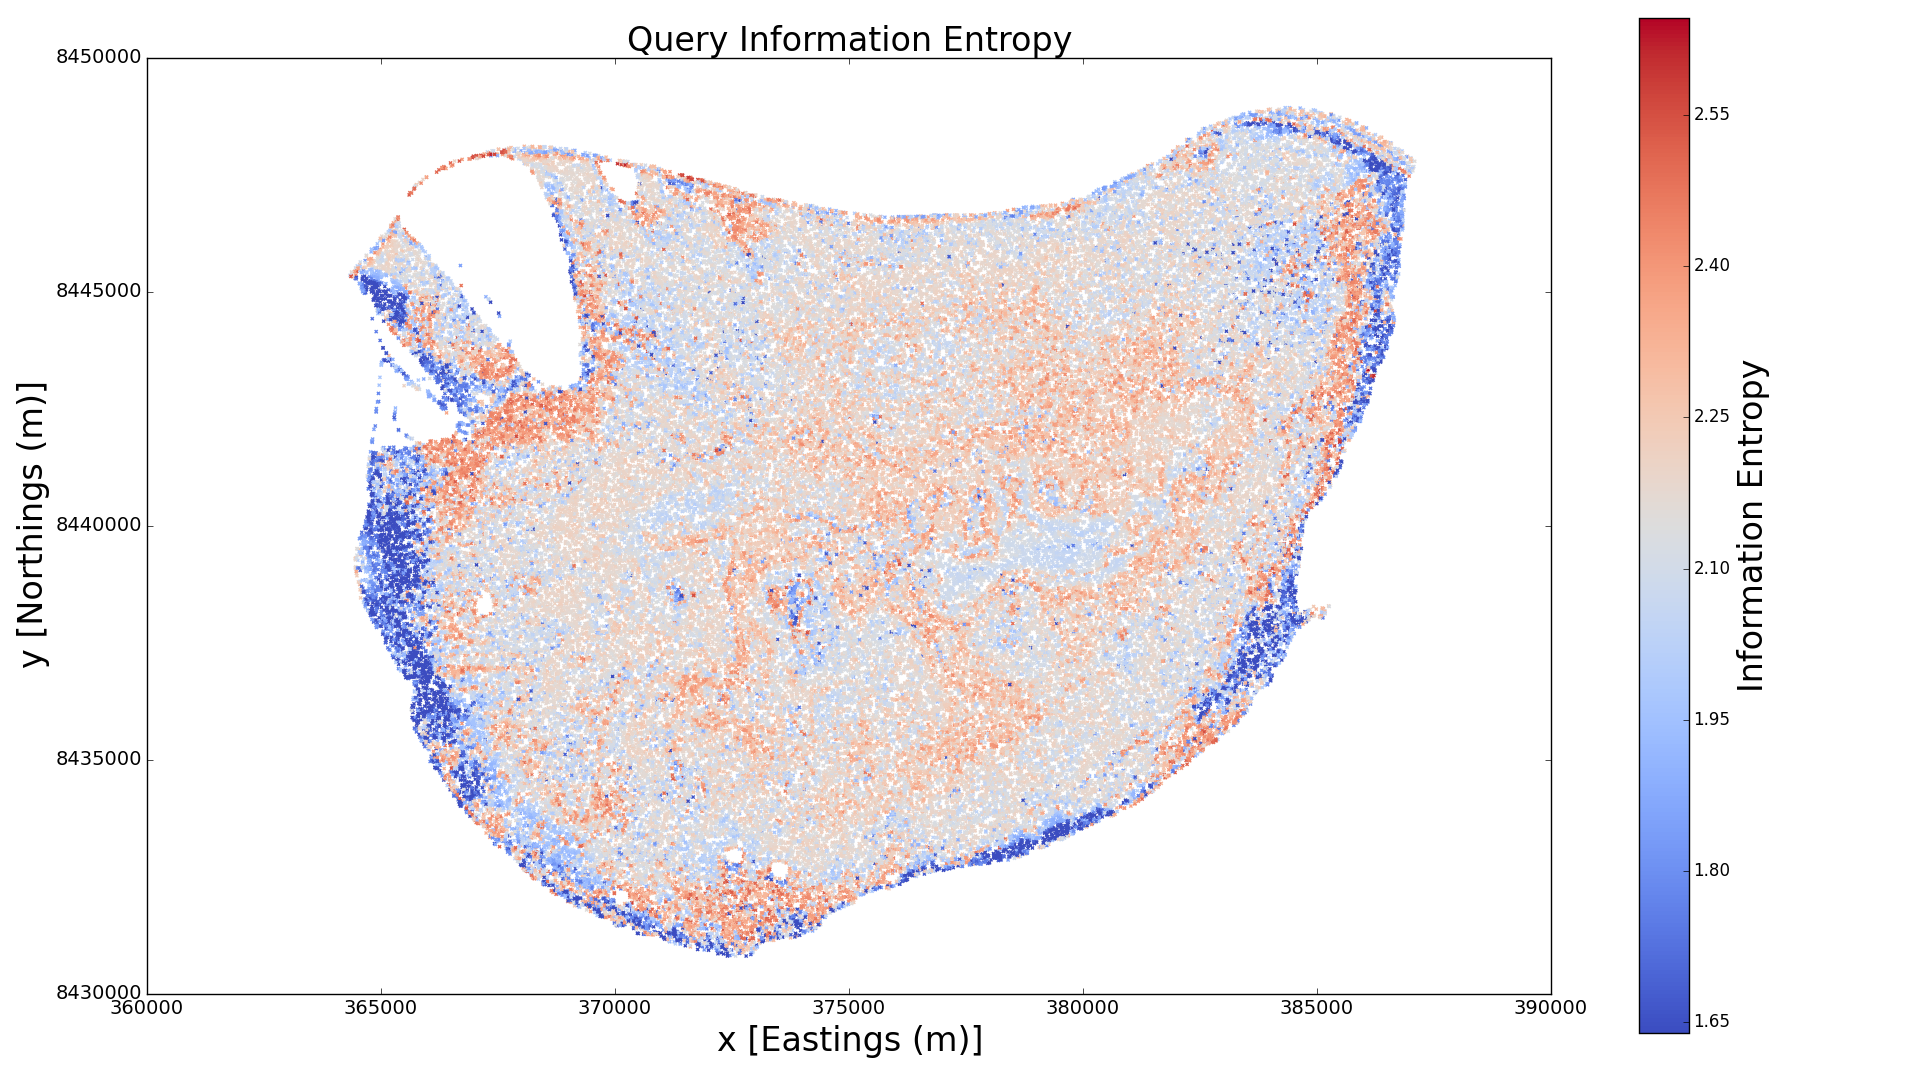
\includegraphics[width = 0.48\linewidth]{Figures/scott_reef_mapping/Figure9.eps}}
			  \subfigure[Linearised Model Differential Entropy]{\label{Figure:ScottReefLinearisedModelDifferentialEntropy}	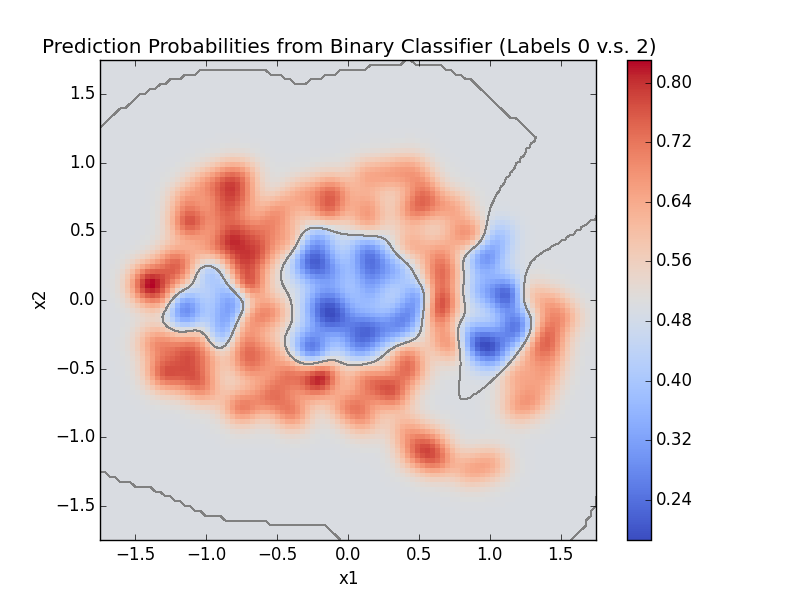
\includegraphics[width = 0.48\linewidth]{Figures//scott_reef_mapping/Figure11.eps}}
			\caption{Scott Reef: Initial Entropy Maps}
			\label{Figure:InitialEntropyMaps}
			\end{figure}
			
			LMDE acquisition, however, emphasizes on the places where the vehicle should first focus on (figure \ref{Figure:ScottReefLinearisedModelDifferentialEntropy}). Comparing Figure \ref{Figure:ScottReefLinearisedModelDifferentialEntropy} with the bathymetric features in Figure \ref{Figure:ScottReefBathymetricFeatures}, the marginalised LMDE is highest at places with the highest and lowest depths (figure \ref{Figure:ScottReefBathymetricFeatures:2}). While Figure \ref{Figure:ScottReefLinearisedModelDifferentialEntropy} only visualises the marginalised entropies, the fact that it is able to emphasize regions with marginalised entropies show that it is better equipped to also discern informative paths in the joint entropy case, leading to LMDE acquisition. Interestingly, the places with highest model variance matches the places with the lowest and highest depths, as it is on the edge of the feature space.
		
			The horizon structure selected for the Scott Reef scenario is 5 km in extent with $n_{p} = 30$ control points. Each control step is therefore $r = \frac{5 \mathrm{km}}{30}$ = 167 meters in length. The turn limit imposed is $\psi_{\mathrm{max}} = \psi_{\mathrm{max}}(r) = 60^{\circ}$. A comparison in performance over a distance of 33.3 km between several acquisition criterion is shown in Figure \ref{Figure:CompareMethods}. Each exploration policy is tested with two distinct two distinct initial locations - (377.5, 8440.0) km and (380.0, 8440.0) km in Eastings-Northings frame. These locations will hereafter be referenced as ``location 1'' and ``location 2'' respectively. The acquisition criterion to be compared are linearised model differential entropy (LMDE), Monte Carlo prediction information entropy (MCPIE), average marginalised prediction information entropy (AMPIE), one step ahead prediction information entropy (GREEDY-PIE), random walk (RANDOM), predetermined spiral path (SPIRAL), and predetermined line segmented paths (LINES). Table \ref{Table:MethodProperties} summarises the essential properties of each exploration policy, revealing that only LMDE and MCPIE acquisition satisfy all desirable requirements.
		
			\begin{table}[t]
				{\footnotesize
				\begin{center}
					\begin{tabular}{ l c c c c c c c }
					\hline
					Policy & LMDE & MCPIE & AMPIE & GREEDY-PIE & RANDOM & LINES & SPIRAL \\
					\hline
					Mutual & Yes & Yes & No & No & No & No & No \\
					Non-Myopic & Yes & Yes & Yes & No & No & Yes & Yes \\
					Informative & Yes & Yes & Yes & Yes & No & No & No \\
					\hline
					\end{tabular}
				\end{center}
				}
		  	\caption{Method Properties and Types}
		  	\label{Table:MethodProperties}			
		  	\end{table}	
		  	

		
%			\begin{figure}[!htbp]
%			\centering
%			  \subfigure[LMDE Acquisition]{\label{Figure:OptimalPathLMDE2} 
%			  	\includegraphics[width = 0.32\linewidth]{Figures/informative_seafloor_exploration/lmde/lde_propose1.eps}
%			  	\includegraphics[width = 0.32\linewidth]{Figures/informative_seafloor_exploration/lmde/lde_propose100.eps}
%			  	\includegraphics[width = 0.32\linewidth]{Figures/informative_seafloor_exploration/lmde/lde_propose200.eps}}
%			  \subfigure[MCPIE Acquisition]{\label{Figure:OptimalPathMCPIE2}	
%			  	\includegraphics[width = 0.32\linewidth]{Figures/informative_seafloor_exploration/mcpie/lde_propose1.eps}
%			  	\includegraphics[width = 0.32\linewidth]{Figures/informative_seafloor_exploration/mcpie/lde_propose100.eps}
%			  	\includegraphics[width = 0.32\linewidth]{Figures/informative_seafloor_exploration/mcpie/lde_propose200.eps}}
%			\caption{Scott Reef: Exploration paths}
%			\label{Figure:OptimalPaths2}
%			\end{figure}
%			
%			\begin{figure}[!htbp]
%			\centering
%			  \subfigure[LMDE Acquisition]{\label{Figure:OptimalPathLMDE3} 
%			  	\includegraphics[width = 0.32\linewidth]{Figures/informative_seafloor_exploration/lmde/pred_propose1.eps}
%			  	\includegraphics[width = 0.32\linewidth]{Figures/informative_seafloor_exploration/lmde/pred_propose100.eps}
%			  	\includegraphics[width = 0.32\linewidth]{Figures/informative_seafloor_exploration/lmde/pred_propose200.eps}}
%			  \subfigure[MCPIE Acquisition]{\label{Figure:OptimalPathMCPIE3}	
%			  	\includegraphics[width = 0.32\linewidth]{Figures/informative_seafloor_exploration/mcpie/pred_propose1.eps}
%			  	\includegraphics[width = 0.32\linewidth]{Figures/informative_seafloor_exploration/mcpie/pred_propose100.eps}
%			  	\includegraphics[width = 0.32\linewidth]{Figures/informative_seafloor_exploration/mcpie/pred_propose200.eps}}
%			\caption{Scott Reef: Exploration paths}
%			\label{Figure:OptimalPaths3}
%			\end{figure}
			
			There are several measures of performance criterion that can be used to measure performance. As the aim is to reduce mapping error, the percentage of misclassification across the map is compared between each method. It is important to understand that the misclassification rate is a rather harsh measure of the prediction performance, as any mismatch in prediction and ground truth is considered a misclassification. Unlike the regression case, there is no inherent measure of proximity in classification targets. For example, classifying \textit{Sand Biota 2} as \textit{Sand Biota 3} is penalised equally as classifying \textit{Sand Biota 2} as \textit{Dense Coral 1}, even though the first case is much more preferable. In this sense, the mapping accuracy is often qualitatively better in reality than the misclassification rate would suggest.
			
			Each method begins with the same scenario, for which the initial misclassification rate with 200 training points is 41.54\% (figure \ref{Figure:ScottReefInitialPredictions}). Table \ref{Table:CompareMethods} shows that, under this performance criterion, LMDE acquisition outperforms other exploration policies, with a final misclassification rate of 16.44\% and 20.38\% for location 1 and 2 respectively at the end of the journey. Methods LINES (20.40\% and 25.05\%) and MCPIE (22.29\% and 27.01\%) follow in performance. The predetermined line segmented paths (LINES) are chosen using after-the-fact knowledge through subjective judgement, and serve as an intuitive anchor for comparison. The MCPIE acquisition approach uses 1000 sample draws from the GP classifier to estimate the joint distribution for 30 control points, and experiences little improvement under misclassification criterion with more samples, as explained in Section \ref{InformativeSeafloorExploration:ComparisonMutualEntropyMeasures:EstimationAccuracy}. Notice that because LMDE acquisition prioritises on decision boundaries, it achieves a lower misclassification rate through appropriately reducing both bias and variance at decision boundaries.
			
			\begin{figure}[!htbp]
			\centering
			  \subfigure[LMDE Acquisition]{\label{Figure:FinalPredictionMapLMDE} \includegraphics[width = 0.48\linewidth]{Figures/informative_seafloor_exploration/lmde/pred200.eps}}
			  \subfigure[MCPIE Acquisition]{\label{Figure:FinalPredictionMapMCPIE}	\includegraphics[width = 0.48\linewidth]{Figures/informative_seafloor_exploration/mcpie/pred200.eps}}
			\caption{Scott Reef: Final Prediction Maps}
			\label{Figure:FinalPredictionMap}
			\end{figure}
		
			Figure \ref{Figure:FinalPredictionMap} shows the final predictions after 33.33 km under LMDE acquisition. The circle represents the horizon extent for which the vehicle considers in at each time step, with the vehicle at the center. The black path with small, coloured empty circles represent the path it has taken. 
					
			\begin{table}[t]
				{\footnotesize
				\begin{center}
					\begin{tabular}{ l c c c c c c c }
					\hline
					Policy & LMDE & MCPIE & AMPIE & GREEDY-PIE & RANDOM & LINES & SPIRAL \\
					\hline
					Location 1 & 16.44 & 22.99 & 32.11 & 43.86 & 34.87 & 20.40 & 33.74 \\
					Location 2 & 20.38 & 27.01 & 40.11 & 37.63 & 35.68 & 25.05 & 43.16 \\
					\hline
					\end{tabular}
				\end{center}
				}
		  	\caption{Final misclassification rate (\%)}
		  	\label{Table:CompareMethods}			
		  	\end{table}	
	  	
			As expected, the paths from the two methods are similar, with LMDE acquisition achieving a misclassification ratio of approximately 6.5\% less. Time lapse plots during the journey is shown in Appendix \ref{Appendix:SeafloorExplorationTimeLapse:Single}, where a more detailed analysis with respect to the prediction information entropy is provided.
			
			From the initial training set shown in Figure \ref{Figure:ScottReefBathymetricFeatures:1}, it is understood that observations are lacking around the edges of the reef. Moreover, Figures \ref{Figure:ScottReefBathymetricFeatures:2} to \ref{Figure:ScottReefBathymetricFeatures:6} reveals that the bathymetric signatures are quite different around the edges. For instance, the bathymetric depth is much lower, and the aspects are much higher. Therefore, it is expected that the AUV should focus on the edges of the reef. Note that from Figure \ref{Figure:ScottReefBathymetricFeatures:1} the shallowest regions of the region is still at least 23 meters in depth, which is still deep enough for exploration.
		
			\begin{figure}[!htbp]
			\centering
				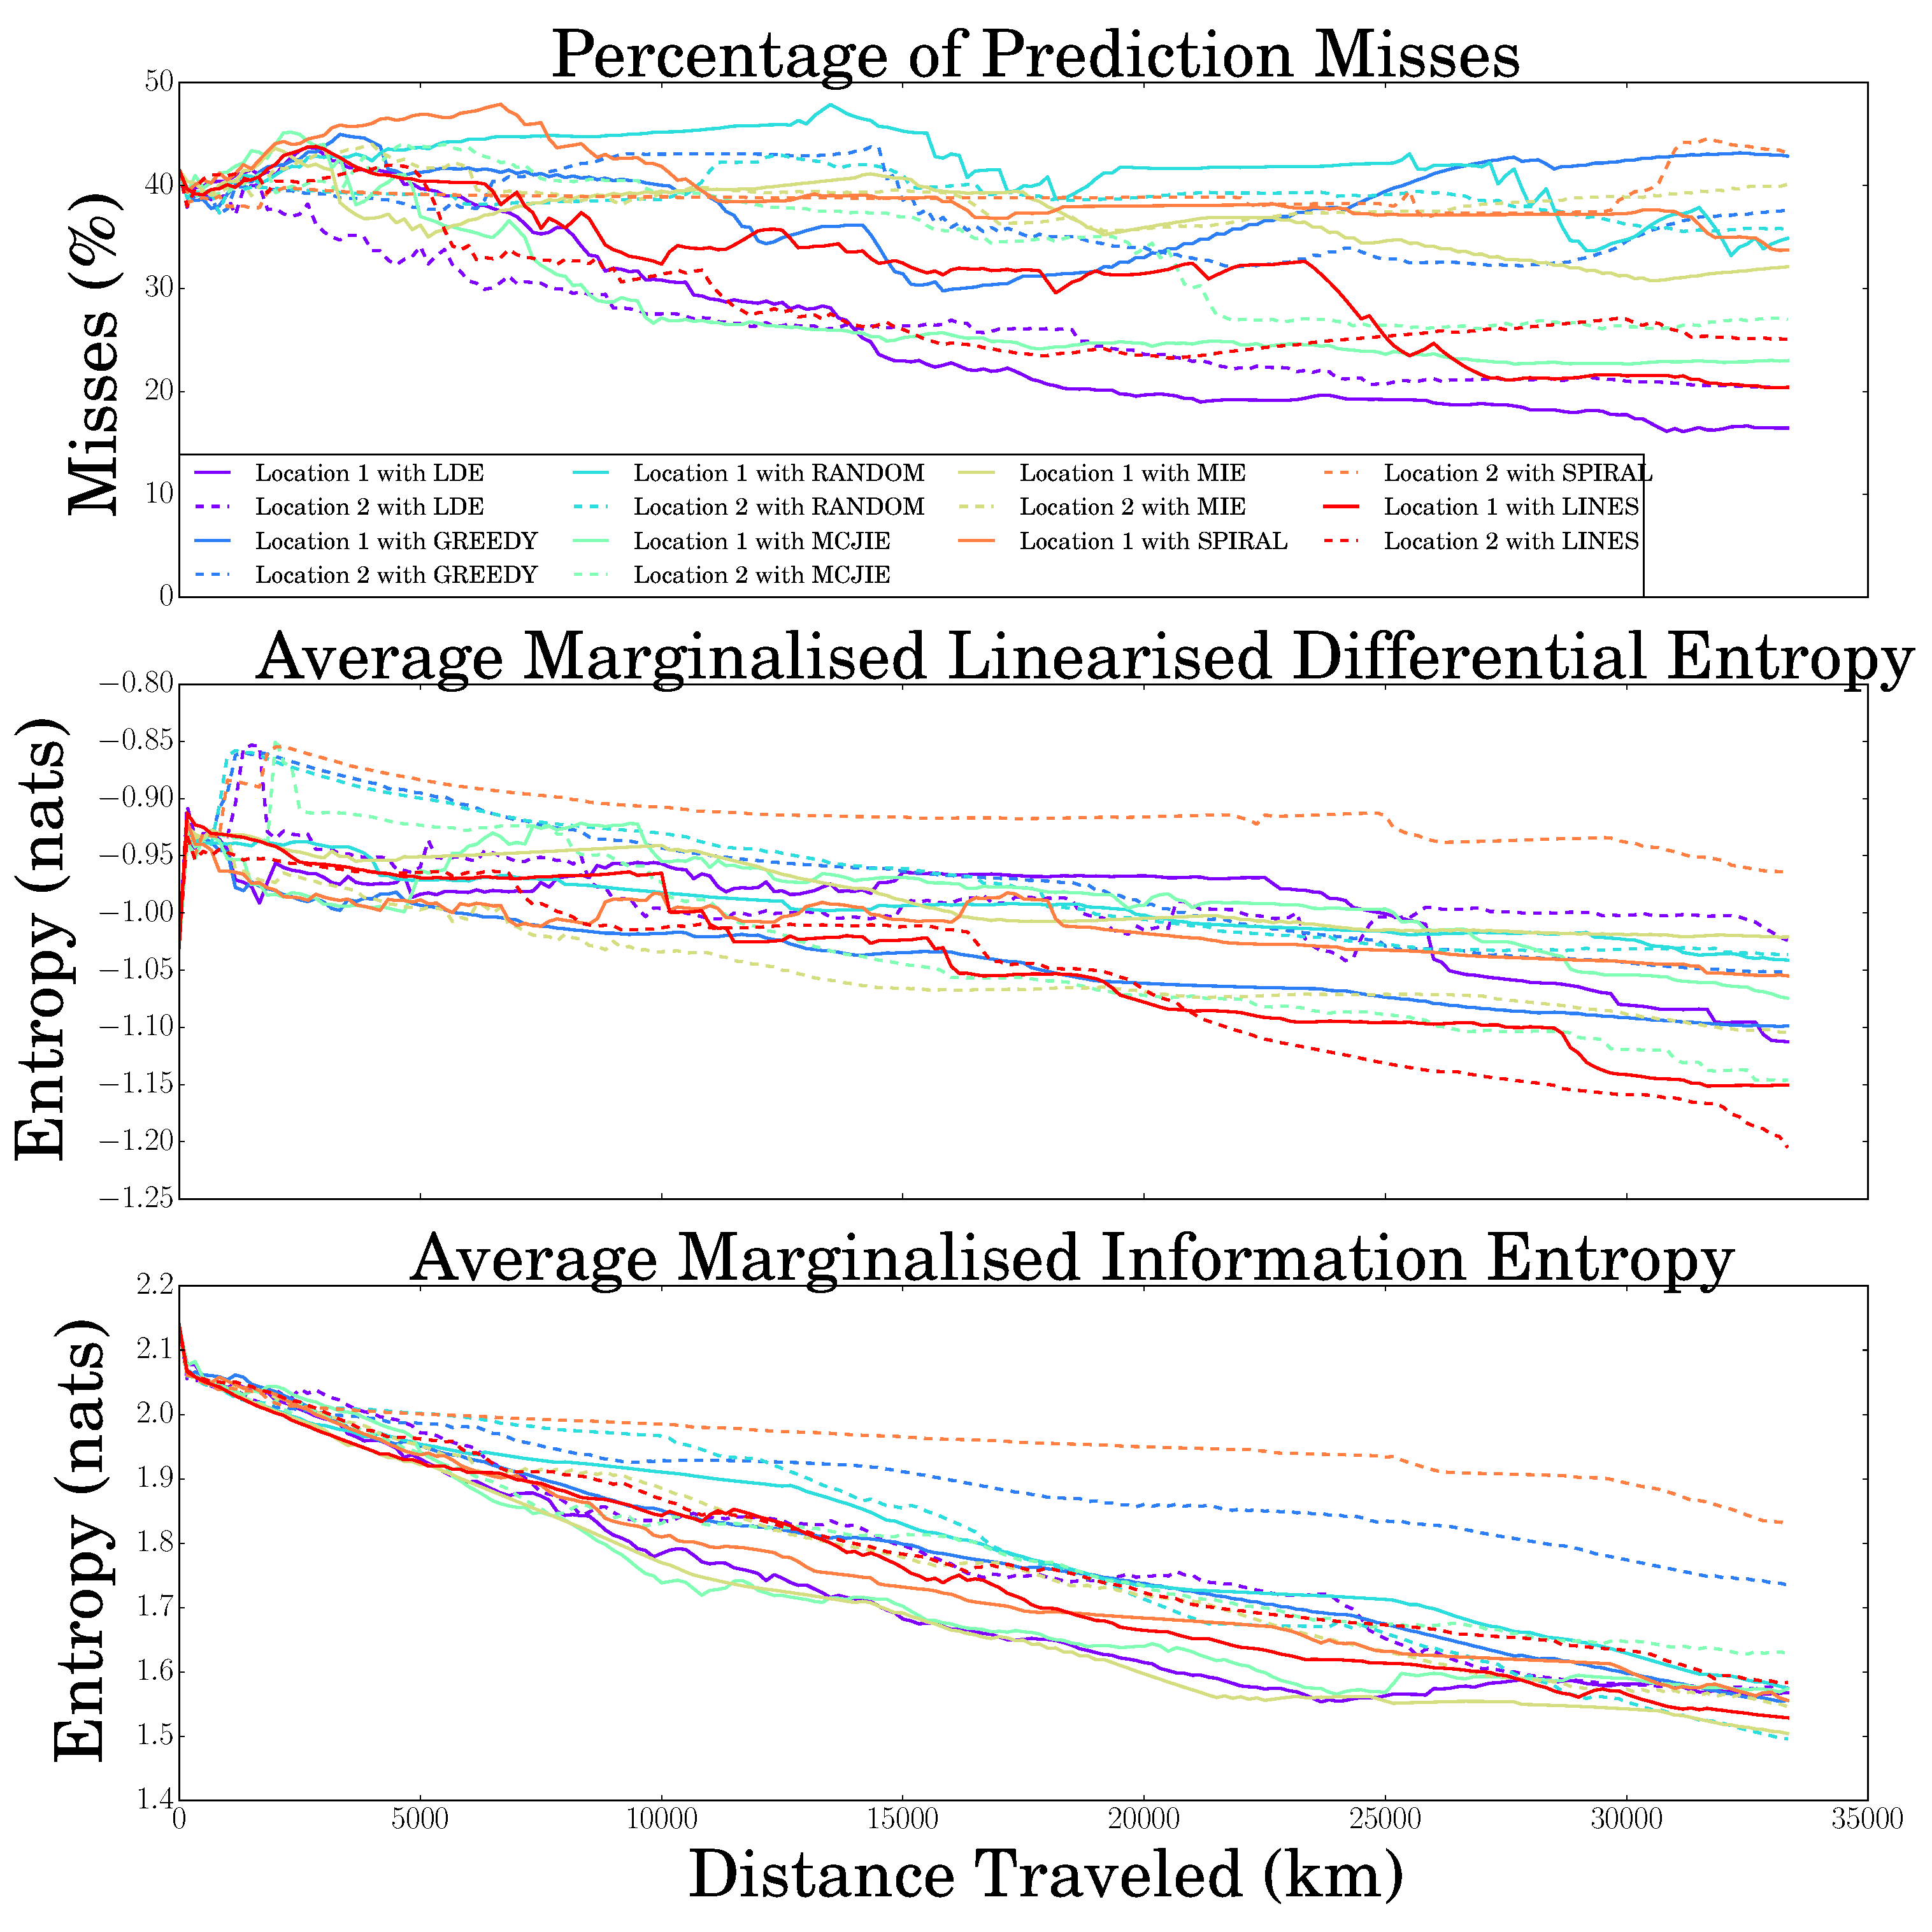
\includegraphics[width = 0.8\linewidth]{Figures/compare_methods.eps}
			\caption{Comparison of informative path planning policies}
			\label{Figure:CompareMethods}
			\end{figure}
				
			Unlike other methods, both the LMDE and MCPIE method take into consideration the mutual information of the proposed path, so that both methods outperform other exploration policies (figure \ref{Figure:CompareMethods} and table \ref{Table:MethodProperties}). This result demonstrates that under a receding horizon formulation, both LMDE and MCPIE acquisitions achieve lower misclassification rate on average than other exploration policies. Furthermore, a receding horizon method achieves lower misclassification rate than myopic approaches under the same acquisition function. Appendix \ref{Appendix:SeafloorExplorationTimeLapse:Single} also verifies the stability of LMDE acquisition through variance analysis.
				
		\subsection{Serial Mission Planning for Seafloor Exploration}
		\label{InformativeSeafloorExploration:ScottReef:SerialMission}
			
			Section \ref{InformativeSeafloorExploration:ScottReef:SingleMission} presented the case for a single mission that is 33.3 km in length. However, in practice the AUV would most likely run out of battery before such long length missions are completed. It is therefore more practical to deploy AUVs on multiple shorter missions, one after the another. Extra flexibility is introduced in this process where the next starting location can be chosen informatively from the observations collected thus far from the previous mission.
			
			As such, this section simulates a serial mission planning process for seafloor exploration, comparing the same set of exploration policies outlined previously. Figure \ref{Figure:ScottReefBathymetricFeatures:1} shows past mission tracks, which are usually more than 8 km in length. The following results assumes that the AUV is equipped with a conservative power supply that allows a mission length of 6.6 km. This distance is also chosen so that five such missions yield a total underwater distance covered of 33.3 km to allow qualitative comparisons against the single mission planning as shown previously. The AUV is to be picked up after each 6.6 km mission through a buoyant vehicle such as a boat, which can sail to the next starting location relatively quickly.
			
			Suppose the AUV is informatively exploring the seafloor using acquisition criterion $I$. After each 6.6 km mission, the AUV chooses the best location $\bvec{p}^{\star}$ to start from for the next mission through finding the region with the highest \textit{regional} acquisition value \eqref{Equation:SerialMissionOptimalLocation}. To allow for fair comparison of the regions, each region is composed of the same number of query points through a standard $k_{NN}$ algorithm.
			
			\begin{equation}
				\begin{aligned}
					\bvec{p}^{\star} &:= \argmax_{\bvec{p} \in \mathcal{P}} I[f_{k}(\bvec{p}) | X, \bvec{y}] \\
					f_{k}(\bvec{p}) &:= \{f_{e}(P) \quad | \quad P = k_{NN}(\bvec{p}, P_{r}, k) \}
				\end{aligned}
			\label{Equation:SerialMissionOptimalLocation}
			\end{equation}
			
			Here, $(X, \bvec{y})$ are the observations collected up to that mission. $k_{NN}(\bvec{p}, P_{r}, k)$ is the $k$-nearest-neighbour algorithm which finds the top $k$ points in $P_{r}$ that is closest to $\bvec{p}$ with respect to the standard Euclidean distance. Furthermore, instead of using the whole seafloor $P_{s}$, a finite subset $P_{r}$ of the $P_{s}$ is used to represent the seafloor to speed up computation. This means that only approximate optimal starting locations can be computed. In practical scenarios, however, this is sufficient.
			
			For the results below, $k = 10$ is chosen. $P_{r}$ is also sampled from $P_{s}$ such that for every point in $P_{r}$, there always exists another point in $P_{r}$ that is less than $100$ meters away. For methods non-informative methods, such as RANDOM, LINES, and SPIRAL, the starting points are then chosen randomly. 
			
			\begin{figure}[!htbp]
			\centering
			  \subfigure{\label{Figure:SerialMissionsSetup:Training}	\includegraphics[width=0.48\linewidth]{Figures/scott_reef_mapping_serial/figure1.eps}}
			  \subfigure{\label{Figure:SerialMissionsSetup:InitialMap}	\includegraphics[width=0.48\linewidth]{Figures/scott_reef_mapping_serial/figure8.eps}}
			  \subfigure{\label{Figure:SerialMissionsSetup:PIE-Map}	\includegraphics[width=0.48\linewidth]{Figures/scott_reef_mapping_serial/figure9.eps}}
			  \subfigure{\label{Figure:SerialMissionsSetup:LMDE-Map}	\includegraphics[width=0.48\linewidth]{Figures/scott_reef_mapping_serial/figure11.eps}}
			\caption{Scott Reef: Serial Missions Setup}
			\label{Figure:SerialMissionsSetup}
			\end{figure}
			
			The added flexibility in serial mission scenario increases performance drastically. To make this more apparent, the initial starting scenario is composed of a minimal training dataset with 17 training points selected randomly from the dataset under the constraint that every training point has a different label (figure \ref{Figure:SerialMissionsSetup:Training}). While it is not necessary to start off with all the possible 17 labels, it enables efficient simulation as it allows corresponding caches to be easily allocated.
			
			The initial prediction map has poor accuracy, with 99.39\% classification miss ratio (figure \ref{Figure:SerialMissionsSetup:InitialMap}), as there are barely any observations to infer upon. Interestingly, the prediction uncertainty (figure \ref{Figure:SerialMissionsSetup:PIE-Map}) and model uncertainty (figure \ref{Figure:SerialMissionsSetup:LMDE-Map}) are almost opposite in trend. Specifically, the effect of bathymetric depth is again the most prominent through comparisons with Figure \ref{Figure:ScottReefBathymetricFeatures:2}. Note that the lowest and highest depths present in the initial training set are 31.69 m and 57.07 m, corresponding to labels \textit{Sand Biota 2} and \textit{Barron Sand 3}. As such, due to a squared exponential kernel, all the regions with depths lower than 31.69 m is predicted with \textit{Sand Biota 2} and all regions with depths higher than 57.07 m is predicted with \textit{Barron Sand 3}, as verified in Figure \ref{Figure:SerialMissionsSetup:InitialMap}. As such, the prediction uncertainty there is low, since there are no other observations to contradict this prediction (figure \ref{Figure:SerialMissionsSetup:PIE-Map}). However, because there is only one observation there, the model uncertainty is high at those points Figure \ref{Figure:SerialMissionsSetup:LMDE-Map}). This again shows that LMDE and PIE are complementary measures of entropy that measures different types of uncertainty.

			For comparison, all methods begin their mission at location 1. While LMDE and MCPIE acquisition produces two different resulting paths, the final prediction map achieved is very similar, with 18.30\% and 21.22\% misclassification ratio respectively (figures \ref{Figure:SerialFinalPredictionMapLMDE} and \ref{Figure:SerialFinalPredictionMapMCPIE}). Other informative exploration policies, AMPIE and GREEDY-PIE, also achieves reasonable mapping rate at 23.21\% and 37.54\% respectively after five 6.6 km missions (figures \ref{Figure:SerialFinalPredictionMapAMPIE} and \ref{Figure:SerialFinalPredictionMapGREEDY}). Compared to the initial scenario with 99.39\% misclassification rate, informative planning are able to achieve efficient mapping under five short missions.
			
			\begin{figure}[!htbp]
			\centering
			  \subfigure[LMDE Acquisition]{\label{Figure:SerialFinalPredictionMapLMDE} \includegraphics[width = 0.48\linewidth]{Figures/informative_seafloor_exploration/serial_lmde/pred199.eps}}
			  \subfigure[MCPIE Acquisition]{\label{Figure:SerialFinalPredictionMapMCPIE} \includegraphics[width = 0.48\linewidth]{Figures/informative_seafloor_exploration/serial_mcpie/pred199.eps}}
			  \subfigure[AMPIE Acquisition]{\label{Figure:SerialFinalPredictionMapAMPIE} \includegraphics[width = 0.48\linewidth]{Figures/informative_seafloor_exploration/serial_ampie/pred199.eps}}
			  \subfigure[GREEDY-PIE Acquisition]{\label{Figure:SerialFinalPredictionMapGREEDY} \includegraphics[width = 0.48\linewidth]{Figures/informative_seafloor_exploration/serial_greedy/pred199.eps}}
			\caption{Scott Reef: Final Prediction Maps}
			\label{Figure:SerialFinalPredictionMap}
			\end{figure}
			
			The same set of exploration policies are then compared in Figure \ref{Figure:SerialCompareMethods}, whose final misclassification rate is summarised in Table \ref{Table:SerialCompareMethods}. In this case, LMDE again outperforms other exploration policies, with MCPIE and AMPIE following closely. Note that this is a typical scenario and does not imply that LMDE acquisition always performs the best, but only most of the time. The performance is also highly dependent on the problem dataset, the ground truth, as well as the GP modelling choices itself. 

			\begin{table}[t]
				{\footnotesize
				\begin{center}
					\begin{tabular}{ l c c c c c c c }
					\hline
					Policy & LMDE & MCPIE & AMPIE & GREEDY-PIE & RANDOM & LINES & SPIRAL \\
					\hline
					Location 1 & 18.30 & 21.22 & 23.21 & 37.54 & 54.63 & 52.54 & 50.06 \\
					\hline
					\end{tabular}
				\end{center}
				}
		  	\caption{Final misclassification rate (\%)}
		  	\label{Table:SerialCompareMethods}
		  	\end{table}	
		  				
			\begin{figure}[!htbp]
			\centering
				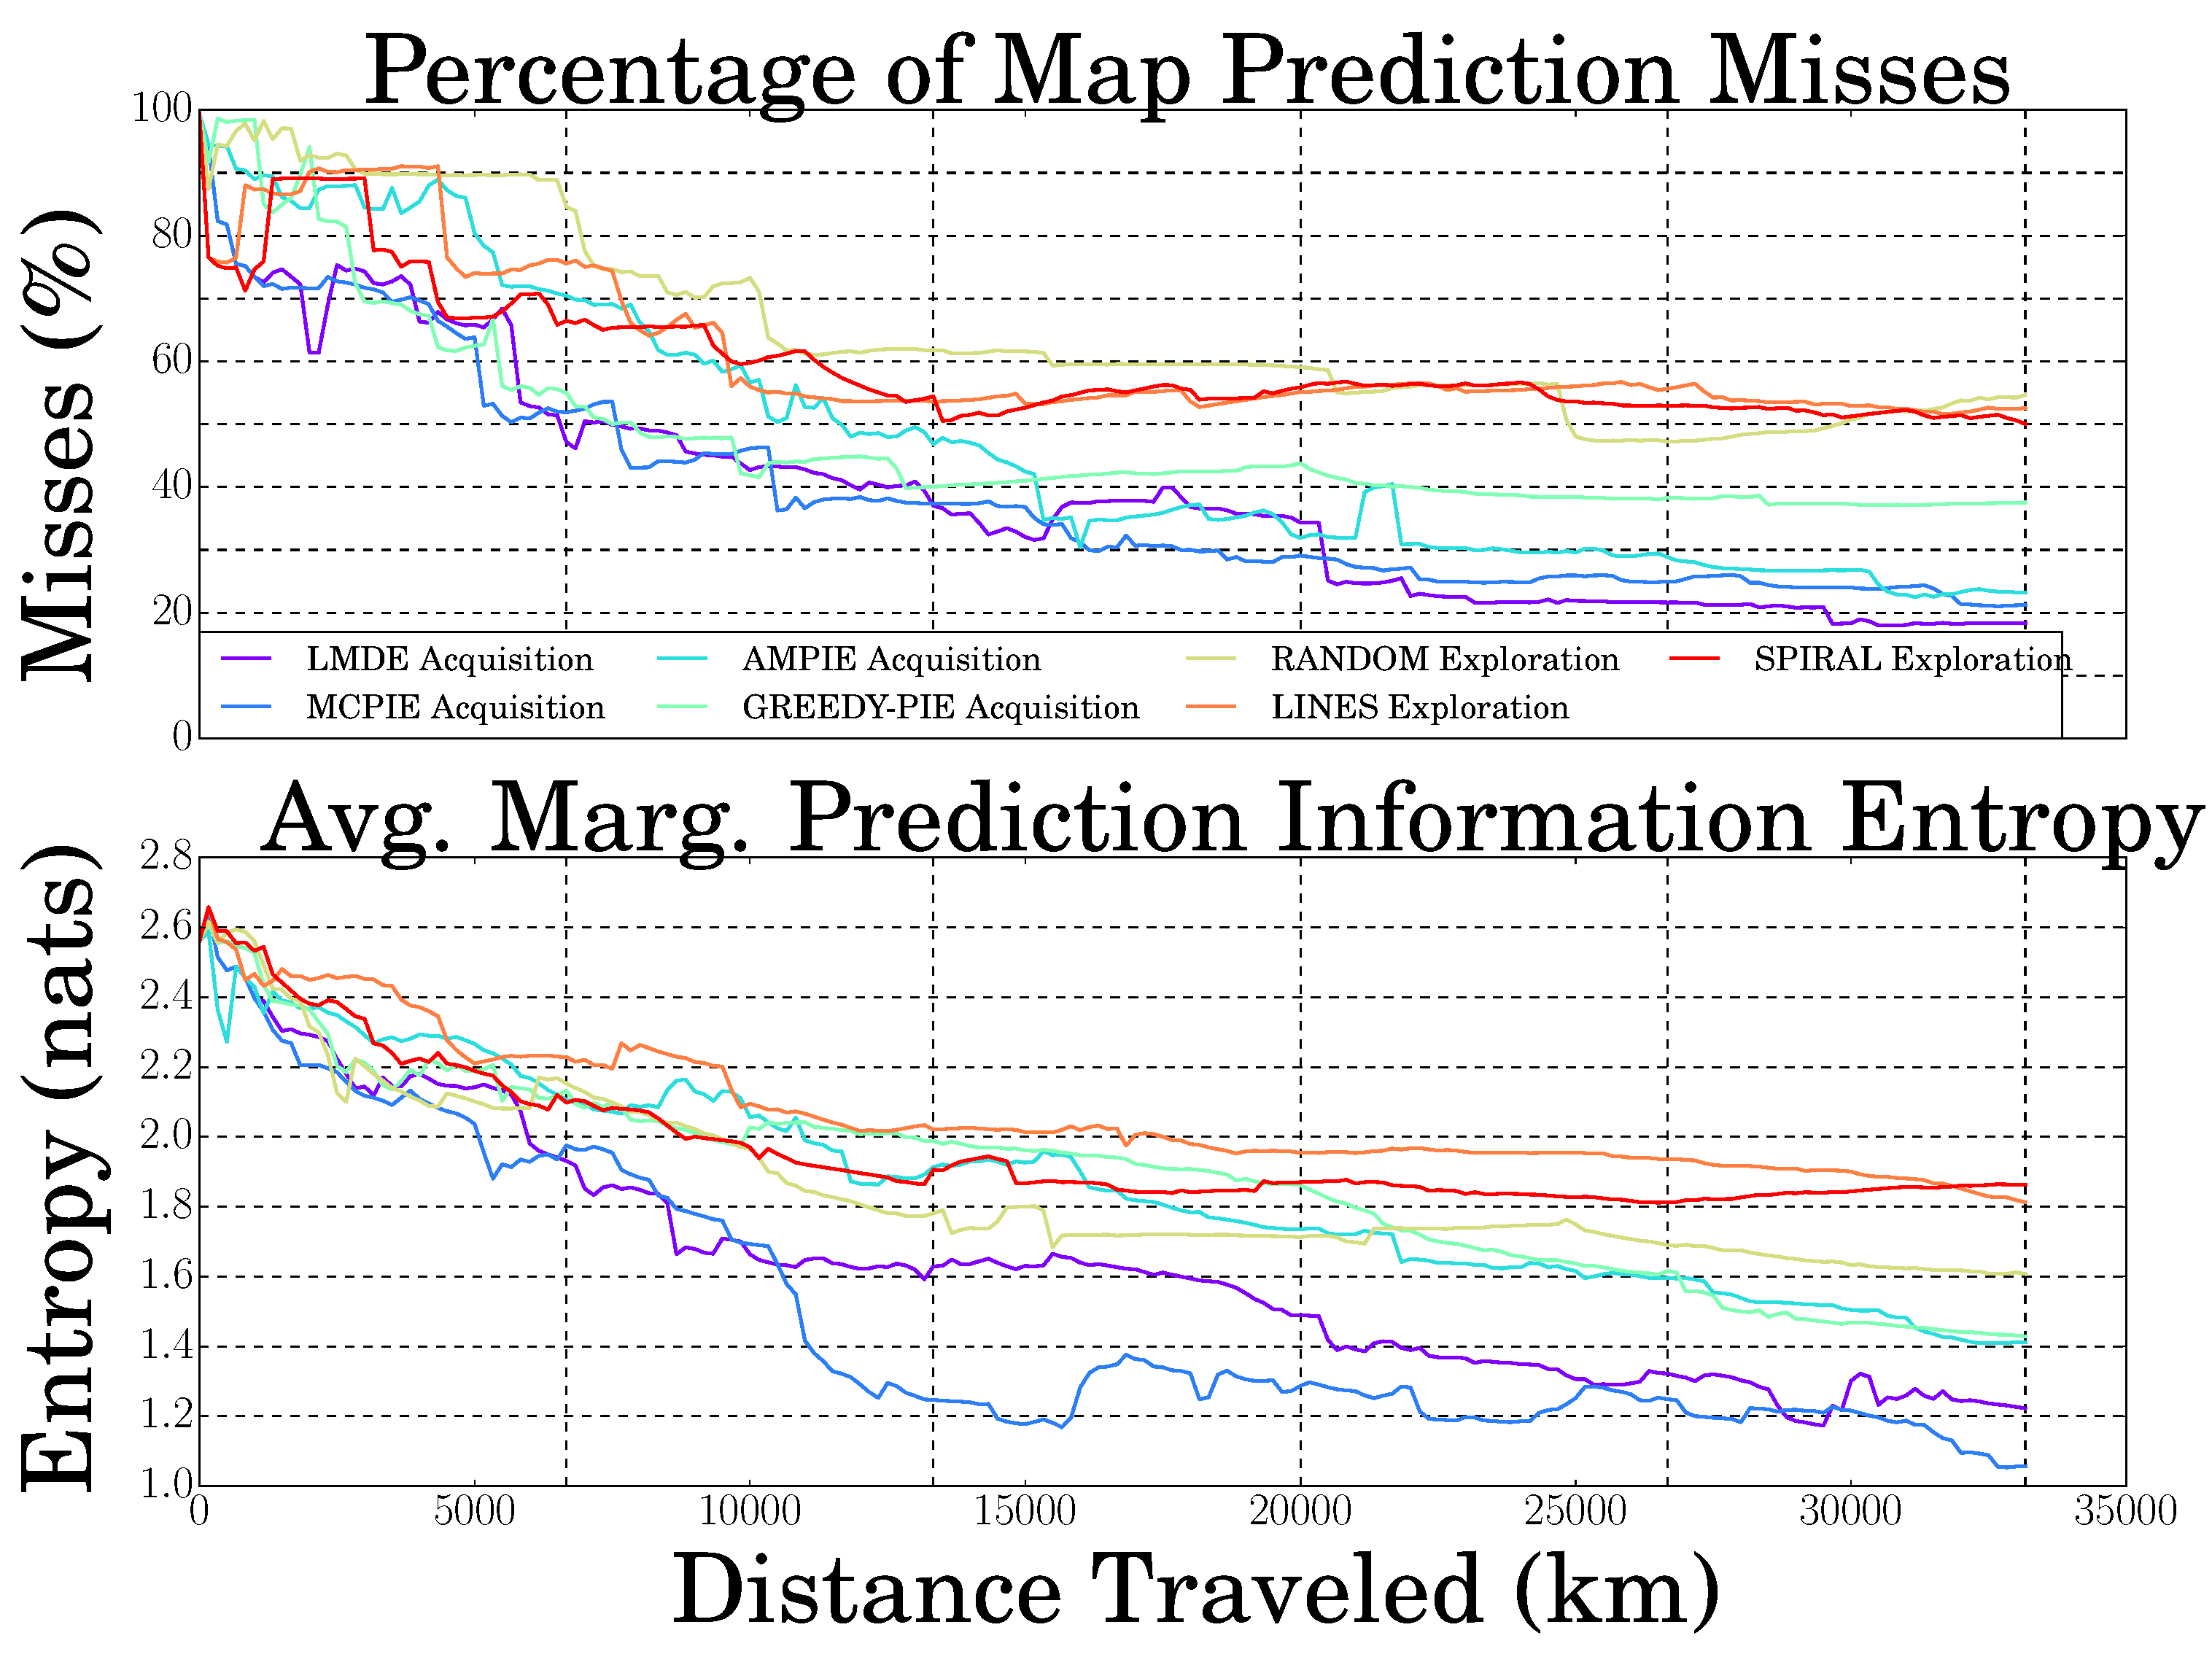
\includegraphics[width = 0.8\linewidth]{Figures/serial_compare_methods.eps}
			\caption{Comparison of informative path planning policies}
			\label{Figure:SerialCompareMethods}
			\end{figure}
						
			Nevertheless, Figure \ref{Figure:SerialCompareMethods} reveals that LMDE and MCPIE acquisitions under the receding horizon framework performs the best. Non-informative methods, however, is only able to achieve no more than 50\% mapping accuracy, with LMDE acquisition achieving more than 30\% mapping accuracy at the end of five missions. As such, simulations verifies the strength of non-myopic, informative path planing policies, and affirms the performance of mutual information measures, LMDE and MCPIE, as acquisition functions.
								
	\section{Summary}
	
		This chapter concludes the work in this thesis through verifying the performance of the two proposed acquisition criteria, LMDE acquisition and MCPIE acquisition. With a proposed receding horizon path planning scheme on the Scott Reef dataset, informative path planning with LMDE acquisition outperforms other methods under a mapping accuracy criteria.
		
		 
		
		
		